% ======== NUOVO: CAPITOLO 3 (pp. 116-120) ========
\chapter{I gruppi di omologia simpliciale}

\section{Simplessi}

\begin{definicion}[Insieme convesso]
Sia $V$ uno spazio vettoriale su $\mathbb{R}$. Un sottoinsieme $C \subseteq V$ si dice \textbf{convesso} se per ogni $x, y \in C$ il segmento
\[
\overline{x,y} = \{ (1-t)x + ty \mid t \in [0,1] \}
\]
\`e contenuto in $C$.
\end{definicion}

\begin{definicion}[Vettori c-indipendenti]
Dato $k \in \mathbb{N}$, i vettori $v_0, \dots, v_k \in V$ si dicono \textbf{c-indipendenti} (``convessamente indipendenti'', detti anche \emph{affinemente indipendenti}) se i $k$ vettori $v_1 - v_0, \dots, v_k - v_0$ sono linearmente indipendenti.
\end{definicion}

\begin{observacion}
La definizione non dipende dal vettore $v_0$ scelto come ``iniziale'': se si sceglie come origine un altro $v_j$, i vettori $v_i - v_j$ ($i \neq j$) sono combinazioni lineari invertibili dei $v_i - v_0$ (infatti $v_i - v_j = (v_i - v_0) - (v_j - v_0)$), quindi sono indipendenti se e solo se lo sono questi.
\end{observacion}

\begin{ejemplo}
\begin{enumerate}
    \item $k = 0$: un singolo vettore $v_0$ \`e (banalmente) c-indipendente, perch\'e la famiglia dei vettori $v_i - v_0$ con $i \geqslant 1$ \`e vuota, e la famiglia vuota \`e linearmente indipendente.
    \item $k = 1$: $v_0, v_1$ sono c-indipendenti $\iff$ $v_1 - v_0$ \`e linearmente indipendente $\iff$ $v_1 - v_0 \neq \bar{0}$ $\iff$ $v_1 \neq v_0$.
    \item $k = 2$: $v_0, v_1, v_2$ sono c-indipendenti $\iff$ $v_1 - v_0, v_2 - v_0$ sono linearmente indipendenti, cio\`e \textbf{non paralleli} $\iff$ $v_0, v_1, v_2$ \textbf{non allineati}.
    \item $k = 3$: $v_0, v_1, v_2, v_3$ sono c-indipendenti $\iff$ $v_1 - v_0, v_2 - v_0, v_3 - v_0$ sono linearmente indipendenti, cio\`e \textbf{non complanari} $\iff$ $v_0, v_1, v_2, v_3$ non sono complanari.
\end{enumerate}
\end{ejemplo}

\begin{observacion}[Nota di correzione]
Negli appunti, al punto 1, si afferma che per $k = 0$ un vettore ``non \`e mai c-indipendente perch\'e $v_0 - v_0 = \bar{0}$''. Questo non \`e coerente con la definizione (per $k=0$ non ci sono vettori $v_i - v_0$ con $i \geqslant 1$, non compare $v_0 - v_0$) e con il seguito: i $0$-simplessi sono proprio i punti. Qui si usa la convenzione standard: ogni punto \`e c-indipendente.
\end{observacion}

\begin{figure}[H]
    \centering
    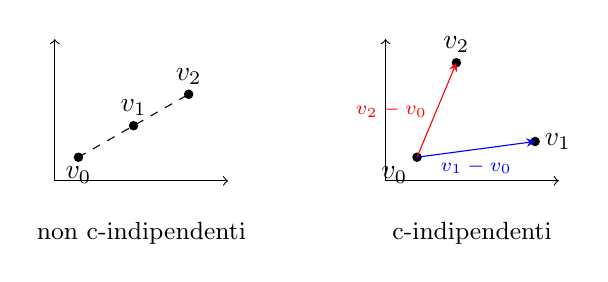
\begin{tikzpicture}[scale=1.0]
        % non c-indipendenti (allineati) e c-indipendenti
        \begin{scope}
            \draw[->] (0,0) -- (2.2,0); \draw[->] (0,0) -- (0,1.8);
            \filldraw (0.3,0.3) circle (1.5pt) node[below] {$v_0$};
            \filldraw (1.0,0.7) circle (1.5pt) node[above] {$v_1$};
            \filldraw (1.7,1.1) circle (1.5pt) node[above] {$v_2$};
            \draw[dashed] (0.3,0.3) -- (1.7,1.1);
            \node[below] at (1.1,-0.4) {\small non c-indipendenti};
        \end{scope}
        \begin{scope}[shift={(4.2,0)}]
            \draw[->] (0,0) -- (2.2,0); \draw[->] (0,0) -- (0,1.8);
            \filldraw (0.4,0.3) circle (1.5pt) node[below left] {$v_0$};
            \filldraw (1.9,0.5) circle (1.5pt) node[right] {$v_1$};
            \filldraw (0.9,1.5) circle (1.5pt) node[above] {$v_2$};
            \draw[blue, ->, >=stealth] (0.4,0.3) -- (1.9,0.5) node[midway, below] {\scriptsize $v_1-v_0$};
            \draw[red, ->, >=stealth] (0.4,0.3) -- (0.9,1.5) node[midway, left] {\scriptsize $v_2-v_0$};
            \node[below] at (1.1,-0.4) {\small c-indipendenti};
        \end{scope}
    \end{tikzpicture}
    \caption{Tre punti sono c-indipendenti se e solo se non sono allineati, cio\`e se $v_1-v_0$ e $v_2-v_0$ non sono paralleli.}
\end{figure}

\begin{definicion}[$k$-piano generato]
Dati $k+1$ vettori c-indipendenti $v_0, \dots, v_k$, l'insieme
\[
\Pi = \left\{ v \in V \;\Big|\; v = \sum_{i=0}^k t_i v_i,\ t_i \in \mathbb{R},\ \sum_{i=0}^k t_i = 1 \right\}
\]
si chiama \textbf{$k$-piano generato} da $v_0, \dots, v_k$.
\end{definicion}

\begin{observacion}
Se $v \in \Pi$, con $v = \sum_{i=0}^k t_i v_i$ e $\sum t_i = 1$, allora
\[
v = t_0 v_0 + \sum_{i=1}^k t_i v_i = \Big(1 - \sum_{i=1}^k t_i\Big) v_0 + \sum_{i=1}^k t_i v_i = v_0 + \sum_{i=1}^k t_i (v_i - v_0).
\]
Quindi $\Pi$ \`e il piano $k$-dimensionale di $V$ passante per $v_0$ e parallelo ai vettori linearmente indipendenti $v_1 - v_0, \dots, v_k - v_0$. In generale $\Pi$ \emph{non} \`e un sottospazio vettoriale, ma un \textbf{sottospazio affine}. Le \emph{trasformazioni affini} di $V$ (le applicazioni $V \to V$ che conservano i sottospazi affini) sono tutte e sole le funzioni $f = \varphi \circ t_v$, con $t_v$ la traslazione $x \mapsto x + v$ e $\varphi \in GL(V)$.
\end{observacion}

\begin{prop}
Sia $V$ di dimensione $n$ e sia $\{e_1, \dots, e_n\}$ una base di $V$. Dati $k+1$ vettori c-indipendenti $v_0, \dots, v_k$ (con $k \leqslant n$), esiste una trasformazione affine $f$ di $V$ tale che $f(\Pi) = \mathcal{L}(e_1, \dots, e_k)$ (il sottospazio generato).
\end{prop}
\begin{proof}
Consideriamo la traslazione $t_{-v_0}$: per l'osservazione precedente, $t_{-v_0}(\Pi) = \mathcal{L}(v_1 - v_0, \dots, v_k - v_0)$, e $v_1 - v_0, \dots, v_k - v_0$ sono linearmente indipendenti. Per il teorema di completamento della base esistono $n-k$ vettori $e'_{k+1}, \dots, e'_n$ di $V$ tali che $\{ v_1 - v_0, \dots, v_k - v_0, e'_{k+1}, \dots, e'_n \}$ sia una base di $V$. Sia $\varphi: V \to V$ lineare tale che $\varphi(v_i - v_0) = e_i$ per $i = 1, \dots, k$ e $\varphi(e'_j) = e_j$ per $j = k+1, \dots, n$. Allora $\varphi \in GL(V)$ (manda una base in una base). Quindi $f = \varphi \circ t_{-v_0}$ \`e una trasformazione affine e
\[
f(\Pi) = \varphi\big( t_{-v_0}(\Pi) \big) = \varphi\big( \mathcal{L}(v_1 - v_0, \dots, v_k - v_0) \big) = \mathcal{L}(e_1, \dots, e_k) . \qquad \square
\]
\end{proof}

\begin{definicion}[Convesso generato]
Sia $V$ uno spazio vettoriale su $\mathbb{R}$ e $X \subseteq V$. Si chiama \textbf{convesso generato} da $X$ il pi\`u piccolo sottoinsieme convesso di $V$ contenente $X$. Dunque $C$ \`e il convesso generato da $X$ se e solo se:
\begin{enumerate}
    \item $C$ \`e convesso;
    \item $X \subseteq C$;
    \item per ogni convesso $C'$ di $V$ con $X \subseteq C'$ si ha $C \subseteq C'$.
\end{enumerate}
\end{definicion}

\begin{observacion}
$C = \bigcap_{C' \text{ convesso},\ X \subseteq C'} C'$ (un'intersezione di convessi \`e convessa).
\end{observacion}

\begin{teo}
Sia $V$ uno spazio vettoriale su $\mathbb{R}$, $k \in \mathbb{N}$ e $v_0, \dots, v_k$ vettori c-indipendenti. Allora il convesso generato da $\{v_0, \dots, v_k\}$ \`e
\[
C = \left\{ v \in V \;\Big|\; v = \sum_{i=0}^k t_i v_i,\ t_i \geqslant 0\ \forall i,\ \sum_{i=0}^k t_i = 1 \right\}.
\]
Inoltre i coefficienti $t_i$ sono univocamente determinati da $v$ (sono le \emph{coordinate baricentriche} di $v$).
\end{teo}

\begin{proof}
Dobbiamo provare che $C$ \`e convesso, che $v_i \in C$ per ogni $i$, e che ogni convesso $C'$ contenente tutti i $v_i$ contiene $C$.

\medskip
\textbf{1. $C$ \`e convesso.} Siano $x, y \in C$, $x = \sum a_i v_i$, $y = \sum b_i v_i$ con $a_i, b_i \geqslant 0$ e $\sum a_i = \sum b_i = 1$. Per ogni $t \in [0,1]$:
\[
(1-t)x + ty = \sum_{i=0}^k \big( (1-t)a_i + t b_i \big) v_i,
\]
con coefficienti $(1-t)a_i + tb_i \geqslant 0$ e $\sum_i \big((1-t)a_i + tb_i\big) = (1-t) + t = 1$. Quindi $(1-t)x + ty \in C$, cio\`e $\overline{x,y} \subseteq C$.

\textbf{2. $v_i \in C$.} Per ogni $i$, $v_i = \sum_j \delta_{ij} v_j$ (delta di Kronecker), con $\delta_{ij} \geqslant 0$ e $\sum_j \delta_{ij} = 1$.

\textbf{3. Minimalit\`a.} Sia $C'$ convesso con $v_0, \dots, v_k \in C'$. Dimostriamo che ogni $v = \sum t_i v_i$ con $t_i \geqslant 0$, $\sum t_i = 1$, appartiene a $C'$, per induzione sul numero $p$ dei coefficienti non nulli.
\begin{itemize}
    \item Se $p = 1$, $v = v_i \in C'$ per qualche $i$.
    \item Supponiamo la tesi vera fino a $p$ e proviamola per $p+1$. Senza perdita di generalit\`a i $p+1$ coefficienti non nulli sono i primi: $v = \sum_{i=0}^{p} t_i v_i$, $t_i > 0$, $\sum_{i=0}^p t_i = 1$. Poich\'e $p+1 \geqslant 2$ coefficienti sono non nulli, $t_p < 1$, e
    \[
    v = \sum_{i=0}^{p-1} t_i v_i + t_p v_p = (1 - t_p) \underbrace{\sum_{i=0}^{p-1} \frac{t_i}{1 - t_p}\, v_i}_{=: w} + t_p v_p .
    \]
    I coefficienti $t_i/(1-t_p)$ sono $> 0$ e hanno somma $\frac{1-t_p}{1-t_p} = 1$, quindi $w$ ha $p$ coefficienti non nulli e, per ipotesi induttiva, $w \in C'$. Allora $v = (1-t_p)w + t_p v_p \in \overline{w, v_p} \subseteq C'$ perch\'e $C'$ \`e convesso.
\end{itemize}
Dunque $C \subseteq C'$ e $C$ \`e il convesso generato.

\textbf{Unicit\`a dei coefficienti.} Se $v = \sum a_i v_i = \sum b_i v_i$ con $\sum a_i = \sum b_i = 1$, allora, poich\'e $\sum_i (a_i - b_i) = 0$,
\[
\bar{0} = \sum_{i=0}^k (a_i - b_i) v_i = \sum_{i=1}^k (a_i - b_i)(v_i - v_0) .
\]
I vettori $v_i - v_0$ sono linearmente indipendenti, quindi $a_i = b_i$ per $i = 1, \dots, k$, e allora $a_0 = 1 - \sum_{i \geqslant 1} a_i = 1 - \sum_{i \geqslant 1} b_i = b_0$\hfill$\square$
\end{proof}

\begin{observacion}
Il convesso generato $C$ \`e contenuto nel $k$-piano $\Pi$ generato dagli stessi vettori ($C \subseteq \Pi$): \`e la parte di $\Pi$ dove i coefficienti sono tutti non negativi.
\end{observacion}


% ======== NUOVO (pp. 121-124) ========
\subsection{Terminologia e notazioni}

Siano $v_0, \dots, v_k \in V$ vettori c-indipendenti. L'insieme convesso generato da $v_0, \dots, v_k$ si chiama \textbf{$k$-simplesso (chiuso)} di vertici $v_0, \dots, v_k$ e si indica con
\[
[v_0, \dots, v_k] = \left\{ v = \sum_{i=0}^k t_i v_i \;\Big|\; t_i \geqslant 0,\ \sum_{i=0}^k t_i = 1 \right\}.
\]
I vettori $v_0, \dots, v_k$ si dicono \textbf{vertici} del $k$-simplesso e $k$ si dice \textbf{dimensione} del simplesso.

\medskip
Per ogni $h \leqslant k$ e per ogni scelta di indici $j_0, \dots, j_h \in \{0, \dots, k\}$ distinti, i vettori $v_{j_0}, \dots, v_{j_h}$ sono c-indipendenti (sottofamiglia di una famiglia c-indipendente) e il simplesso $[v_{j_0}, \dots, v_{j_h}] \subseteq [v_0, \dots, v_k]$ si dice \textbf{faccia $h$-dimensionale chiusa} di $[v_0, \dots, v_k]$. In particolare, fissato $j \in \{0, \dots, k\}$,
\[
[v_0, \dots, \widehat{v_j}, \dots, v_k] = [v_0, \dots, v_{j-1}, v_{j+1}, \dots, v_k]
\]
(il cappuccio indica che $v_j$ \`e omesso) si dice \textbf{faccia $(k-1)$-dimensionale chiusa opposta a $v_j$}.

\medskip
L'insieme
\[
(s) = (v_0, \dots, v_k) = \left\{ v \in V \;\Big|\; v = \sum_{i=0}^k t_i v_i,\ t_i > 0\ \forall i,\ \sum_{i=0}^k t_i = 1 \right\}
\]
(con coefficienti \emph{strettamente} positivi) si chiama \textbf{$k$-simplesso aperto} determinato da $v_0, \dots, v_k$. Per ogni $h \leqslant k$ e $j_0, \dots, j_h$ distinti, $(v_{j_0}, \dots, v_{j_h})$ si dice \textbf{faccia $h$-dimensionale aperta} del $k$-simplesso (chiuso) $[s] = [v_0, \dots, v_k]$. Chiaramente $(s) \subseteq [s]$.

\begin{ejercicio*}
\begin{enumerate}
    \item Dimostrare che $(s)$ \`e convesso.
    \item Dimostrare che $[s]$ \`e l'unione \emph{disgiunta} delle sue facce aperte $(s')$.
\end{enumerate}
\end{ejercicio*}
\textit{Soluzione.} (1) Se $x = \sum a_i v_i$ e $y = \sum b_i v_i$ hanno coefficienti $a_i, b_i > 0$, allora $(1-t)x + ty = \sum ((1-t)a_i + t b_i) v_i$ ha coefficienti $(1-t)a_i + t b_i > 0$ per ogni $t \in [0,1]$ (perch\'e almeno uno tra $1-t$ e $t$ \`e positivo) e somma $1$.
(2) Se $v = \sum t_i v_i \in [s]$, sia $J = \{ i \mid t_i > 0 \}$: allora $v$ appartiene alla faccia aperta $(v_j)_{j \in J}$. Poich\'e i coefficienti sono univocamente determinati (teorema precedente), $J$ \`e univocamente determinato da $v$, quindi $v$ sta in \emph{una sola} faccia aperta: l'unione \`e disgiunta.

\begin{ejemplo}
\begin{enumerate}
    \item \textbf{$k = 0$.} Impropriamente si chiama $0$-simplesso il pi\`u piccolo convesso contenente $v_0$, cio\`e $\{v_0\}$. Osserviamo che $k = 0$ \`e l'unico caso in cui il simplesso aperto e quello chiuso coincidono: $[v_0] = (v_0) = \{v_0\}$.
    \item \textbf{$k = 1$.} Siano $v_0, v_1$ c-indipendenti ($v_0 \neq v_1$). Allora
    \[
    [v_0, v_1] = \{ v \mid v = (1-t_1)v_0 + t_1 v_1,\ t_1 \geqslant 0,\ 1 - t_1 \geqslant 0 \} = \{ (1-t)v_0 + t v_1 \mid 0 \leqslant t \leqslant 1 \} = \overline{v_0 v_1},
    \]
    il \textbf{segmento} di estremi $v_0, v_1$. Inoltre $(v_0, v_1) = \{ (1-t)v_0 + t v_1 \mid 0 < t < 1 \}$ e
    \[
    [v_0, v_1] = (v_0, v_1) \sqcup (v_0) \sqcup (v_1).
    \]
    \item \textbf{$k = 2$.} Se $v_0, v_1, v_2$ non sono allineati, $[v_0, v_1, v_2]$ \`e il \textbf{triangolo pieno} di vertici $v_0, v_1, v_2$.
    \item \textbf{$k = 3$.} Se $v_0, v_1, v_2, v_3$ non sono complanari, $[v_0, v_1, v_2, v_3]$ \`e il \textbf{tetraedro pieno} di vertici $v_0, v_1, v_2, v_3$.
\end{enumerate}
\end{ejemplo}

\begin{figure}[H]
    \centering
    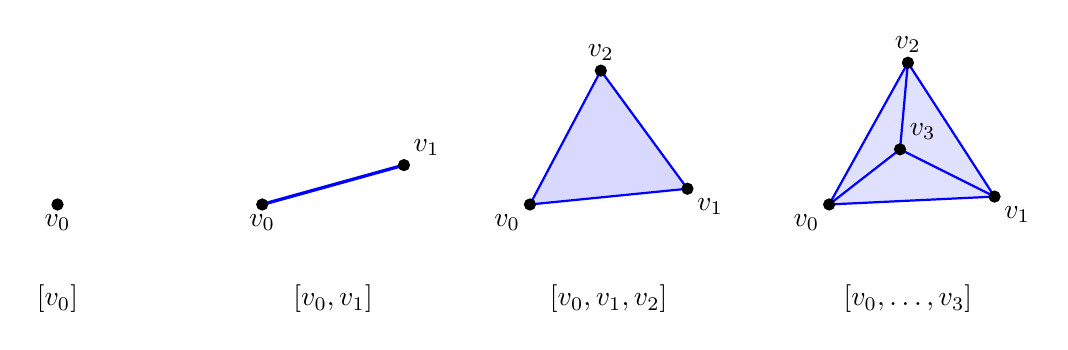
\begin{tikzpicture}[scale=1.0]
        % 0-simplesso
        \begin{scope}
            \filldraw (0,0) circle (2pt) node[below] {$v_0$};
            \node at (0,-1.2) {$[v_0]$};
        \end{scope}
        % 1-simplesso
        \begin{scope}[shift={(2.6,0)}]
            \draw[very thick, blue] (0,0) -- (1.8,0.5);
            \filldraw (0,0) circle (2pt) node[below] {$v_0$};
            \filldraw (1.8,0.5) circle (2pt) node[above right] {$v_1$};
            \node at (0.9,-1.2) {$[v_0, v_1]$};
        \end{scope}
        % 2-simplesso
        \begin{scope}[shift={(6.0,0)}]
            \fill[blue!15] (0,0) -- (2,0.2) -- (0.9,1.7) -- cycle;
            \draw[thick, blue] (0,0) -- (2,0.2) -- (0.9,1.7) -- cycle;
            \filldraw (0,0) circle (2pt) node[below left] {$v_0$};
            \filldraw (2,0.2) circle (2pt) node[below right] {$v_1$};
            \filldraw (0.9,1.7) circle (2pt) node[above] {$v_2$};
            \node at (1.0,-1.2) {$[v_0, v_1, v_2]$};
        \end{scope}
        % 3-simplesso
        \begin{scope}[shift={(9.8,0)}]
            \fill[blue!12] (0,0) -- (2.1,0.1) -- (1.0,1.8) -- cycle;
            \draw[thick, blue] (0,0) -- (2.1,0.1) -- (1.0,1.8) -- cycle;
            \draw[thick, blue] (0.9,0.7) -- (0,0);
            \draw[thick, blue] (0.9,0.7) -- (2.1,0.1);
            \draw[thick, blue] (0.9,0.7) -- (1.0,1.8);
            \filldraw (0,0) circle (2pt) node[below left] {$v_0$};
            \filldraw (2.1,0.1) circle (2pt) node[below right] {$v_1$};
            \filldraw (1.0,1.8) circle (2pt) node[above] {$v_2$};
            \filldraw (0.9,0.7) circle (2pt) node[above right] {$v_3$};
            \node at (1.0,-1.2) {$[v_0, \dots, v_3]$};
        \end{scope}
    \end{tikzpicture}
    \caption{I simplessi di dimensione $0$, $1$, $2$, $3$: punto, segmento, triangolo pieno, tetraedro pieno.}
\end{figure}

\begin{teo}
Sia $[s] = [v_0, \dots, v_k]$ un $k$-simplesso e sia fissato $j \in \{0, \dots, k\}$. Allora
\[
v \in [s] \iff \exists\, w \in [v_0, \dots, \widehat{v_j}, \dots, v_k] \ : \ v \in \overline{w, v_j}.
\]
In parole: $[s]$ \`e l'unione dei segmenti che congiungono $v_j$ con i punti della faccia opposta (un ``cono'' di vertice $v_j$ sulla faccia opposta).
\end{teo}
\begin{proof}
($\Leftarrow$) \`E banale: $v_j \in [s]$, la faccia opposta $[v_0, \dots, \widehat{v_j}, \dots, v_k] \subseteq [s]$, quindi $w \in [s]$ e, essendo $[s]$ convesso, $\overline{w, v_j} \subseteq [s]$.

($\Rightarrow$) Senza perdita di generalit\`a $j = k$. Sia $v \in [s]$: $v = \sum_{i=0}^k t_i v_i$, $t_i \geqslant 0$, $\sum t_i = 1$. Se $v = v_k$, ogni $w$ va bene ($v \in \overline{w, v_k}$). Sia quindi $v \neq v_k$: allora $t_k \neq 1$, cio\`e $t_k < 1$, e
\[
v = \sum_{i=0}^{k-1} t_i v_i + t_k v_k = (1 - t_k) \underbrace{\sum_{i=0}^{k-1} \frac{t_i}{1 - t_k}\, v_i}_{=: w} + t_k v_k .
\]
I coefficienti $t_i/(1-t_k)$ sono $\geqslant 0$ e hanno somma $\frac{1-t_k}{1-t_k} = 1$, quindi $w \in [v_0, \dots, v_{k-1}] = [v_0, \dots, v_{k-1}, \widehat{v_k}]$ e $v = (1-t_k)w + t_k v_k \in \overline{w, v_k}$\hfill$\square$
\end{proof}

\begin{definicion}[Coordinate baricentriche e baricentro]
Sia $[s] = [v_0, \dots, v_k]$ un $k$-simplesso, cio\`e per ogni $v \in [s]$ si ha $v = \sum_{i=0}^k t_i v_i$ con $t_i \geqslant 0$, $\sum t_i = 1$. I coefficienti $(t_0, \dots, t_k)$ sono univocamente determinati e si chiamano \textbf{coordinate baricentriche} di $v$ in $[s]$. Il punto $b = \left( \frac{1}{k+1}, \dots, \frac{1}{k+1} \right)$ (cio\`e $b = \frac{1}{k+1} \sum_i v_i$) si chiama \textbf{baricentro} del $k$-simplesso $[s]$.
\end{definicion}

\begin{intuizione}
Le coordinate baricentriche dicono ``quanto peso'' si d\`a a ciascun vertice per ottenere il punto $v$: $v$ \`e il baricentro di masse $t_0, \dots, t_k$ poste sui vertici. Il baricentro $b$ \`e il caso in cui tutti i pesi sono uguali.
\end{intuizione}


% ======== NUOVO (pp. 125-126, 22/10/2026) ========
\subsection{Il baricentro di un simplesso}

\begin{ejemplo}
Sia $[s] = [v_0, \dots, v_k]$ e $b = \left( \frac{1}{k+1}, \dots, \frac{1}{k+1} \right)$ il suo baricentro.
\begin{itemize}
    \item $k = 0$: $[v_0] = (v_0) = \{v_0\} = \{b\}$.
    \item $k = 1$: $[v_0, v_1] = \overline{v_0 v_1}$ e $b = \frac12 v_0 + \frac12 v_1$: $b$ \`e il \textbf{punto medio} del segmento, che lo divide in due parti uguali.
    \item $k = 2$: $[v_0, v_1, v_2]$ e
    \[
    b = \tfrac13 v_0 + \tfrac13 v_1 + \tfrac13 v_2 = \tfrac13 v_0 + \tfrac23\left( \tfrac12 v_1 + \tfrac12 v_2 \right) .
    \]
    Quindi $b$ \`e il baricentro del triangolo, cio\`e il punto di intersezione delle sue \textbf{mediane}; $b$ divide ciascuna mediana in due segmenti che stanno in rapporto $1 : 2$.
    \item $k = 3$: $[v_0, v_1, v_2, v_3]$ e
    \[
    b = \tfrac14 v_0 + \tfrac14 v_1 + \tfrac14 v_2 + \tfrac14 v_3 = \tfrac14 v_0 + \tfrac34\left( \tfrac13 v_1 + \tfrac13 v_2 + \tfrac13 v_3 \right).
    \]
    Quindi $b$ \`e il baricentro del tetraedro, cio\`e il punto di intersezione dei segmenti che congiungono ciascun vertice con il baricentro della faccia ad esso opposta, e li divide in due segmenti in rapporto $1 : 3$.
\end{itemize}
\end{ejemplo}

\begin{figure}[H]
    \centering
    \begin{tikzpicture}[scale=1.4]
        \coordinate (v0) at (0,0);
        \coordinate (v1) at (3,0);
        \coordinate (v2) at (1.1,2.4);
        \coordinate (m0) at ($(v1)!0.5!(v2)$);
        \coordinate (m1) at ($(v0)!0.5!(v2)$);
        \coordinate (m2) at ($(v0)!0.5!(v1)$);
        \draw[thick, fill=blue!8] (v0) -- (v1) -- (v2) -- cycle;
        \draw[gray] (v0) -- (m0); \draw[gray] (v1) -- (m1); \draw[gray] (v2) -- (m2);
        \coordinate (bb) at (1.3667,0.8);
        \filldraw[red] (bb) circle (2pt) node[above right] {$b$};
        \filldraw (v0) circle (1.5pt) node[below left] {$v_0$};
        \filldraw (v1) circle (1.5pt) node[below right] {$v_1$};
        \filldraw (v2) circle (1.5pt) node[above] {$v_2$};
    \end{tikzpicture}
    \caption{Il baricentro $b$ di un triangolo \`e l'intersezione delle mediane e le divide in rapporto $1:2$.}
\end{figure}

\begin{prop}
Sia $[s] = [v_0, \dots, v_k]$ un $k$-simplesso e $b$ il suo baricentro. Allora $b$ \`e il punto di intersezione dei segmenti che congiungono ciascun vertice $v_j$ con il baricentro della faccia ad esso opposta, e divide ciascuno di questi segmenti in due parti che stanno in rapporto $1 : k$ (la parte verso la faccia \`e $1/(k+1)$ del segmento, la parte verso il vertice \`e $k/(k+1)$).
\end{prop}
\begin{proof}
Per simmetria basta considerare $v_0$. Il baricentro della faccia opposta $[v_1, \dots, v_k]$ \`e $b_0' = \frac{1}{k}(v_1 + \dots + v_k)$ e
\[
b = \frac{1}{k+1} v_0 + \dots + \frac{1}{k+1} v_k = \frac{1}{k+1} v_0 + \frac{k}{k+1} \left( \frac1k v_1 + \dots + \frac1k v_k \right) = \frac{1}{k+1} v_0 + \frac{k}{k+1}\, b_0' .
\]
Dunque $b$ sta sul segmento $\overline{v_0 b_0'}$ e $b - v_0 = \frac{k}{k+1}(b_0' - v_0)$: la distanza da $v_0$ \`e i $k/(k+1)$ del segmento, quella da $b_0'$ \`e $1/(k+1)$, quindi $|b b_0'| : |v_0 b| = 1 : k$. Lo stesso calcolo vale per ogni vertice $v_j$, e il punto $b$, avendo coordinate baricentriche $\frac{1}{k+1}$ tutte uguali, \`e lo stesso in ogni caso\hfill$\square$
\end{proof}


% ======== NUOVO (pp. 127-130) ========
\section{Complessi simpliciali}

\begin{definicion}[Complesso simpliciale]
Si chiama \textbf{complesso simpliciale} (euclideo finito) un qualsiasi insieme \emph{finito} $K$ di simplessi \emph{aperti} di $\mathbb{R}^n$ tale che:
\begin{enumerate}
    \item[1)] se $(s) \in K$, allora $K$ contiene ogni faccia aperta di $(s)$;
    \item[2)] per ogni $(s), (s') \in K$: $(s) = (s')$ oppure $(s) \cap (s') = \varnothing$.
\end{enumerate}
\end{definicion}

\begin{intuizione}
Un complesso simpliciale \`e un ``oggetto geometrico costruito incollando punti, segmenti, triangoli, tetraedri, \dots'' in modo coerente: (1) se c'\`e un triangolo ci sono anche i suoi lati e i suoi vertici; (2) due simplessi distinti non si sovrappongono (si incontrano al pi\`u lungo facce comuni, che sono a loro volta elementi di $K$).
\end{intuizione}

\begin{definicion}[Dimensione e sostegno]
La \textbf{dimensione} del complesso simpliciale $K$ \`e $\dim K = \max_{(s) \in K} \dim [s]$. Si chiama \textbf{sostegno} di $K$ l'insieme
\[
|K| = \bigcup_{(s) \in K} (s) \subseteq \mathbb{R}^n .
\]
\end{definicion}

\begin{observacion}
\textbf{Non confondere $K$ e $|K|$!} $K$ \`e un insieme \emph{finito} di simplessi aperti (dato combinatorio), mentre $|K|$ \`e un sottoinsieme di $\mathbb{R}^n$ (lo spazio topologico). Lo stesso sostegno pu\`o essere il sostegno di complessi diversi.
\end{observacion}

\begin{ejemplo}[Decomposizione simpliciale di un simplesso chiuso]
Sia $[s] = [v_0, \dots, v_k]$ un $k$-simplesso chiuso. Allora $K = \{ (s') \mid (s') \text{ faccia aperta di } [s] \}$ \`e un complesso simpliciale di dimensione $k$ e sostegno $|K| = [s]$ (per l'esercizio precedente $[s]$ \`e l'unione disgiunta delle sue facce aperte). Un $k$-simplesso ha $2^{k+1} - 1$ facce aperte non vuote:
\begin{itemize}
    \item $k = 1$: $[v_0, v_1] = \overline{v_0 v_1}$, $K = \{ (v_0), (v_1), (v_0, v_1) \}$ (3 elementi).
    \item $k = 2$: $[v_0, v_1, v_2]$, $K = \{ (v_0), (v_1), (v_2), (v_0, v_1), (v_0, v_2), (v_1, v_2), (v_0, v_1, v_2) \}$ (7 elementi).
    \item $k = 3$: $[v_0, v_1, v_2, v_3]$, $K$ ha $4$ vertici, $6$ spigoli, $4$ facce triangolari e $1$ tetraedro aperto: $15$ elementi.
\end{itemize}
Cos\`i, il segmento chiuso $[v_0, v_1]$ \`e il sostegno di $K = \{ (v_0), (v_1), (v_0,v_1) \}$.
\end{ejemplo}

\begin{figure}[H]
    \centering
    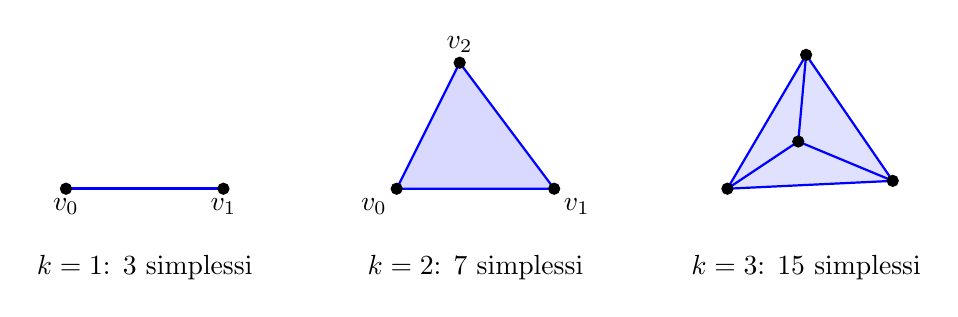
\begin{tikzpicture}[scale=1.0]
        \begin{scope}
            \draw[very thick, blue] (0,0) -- (2,0);
            \filldraw (0,0) circle (2pt) node[below] {$v_0$};
            \filldraw (2,0) circle (2pt) node[below] {$v_1$};
            \node at (1,-1.0) {$k=1$: 3 simplessi};
        \end{scope}
        \begin{scope}[shift={(4.2,0)}]
            \fill[blue!15] (0,0) -- (2,0) -- (0.8,1.6) -- cycle;
            \draw[thick, blue] (0,0) -- (2,0) -- (0.8,1.6) -- cycle;
            \filldraw (0,0) circle (2pt) node[below left] {$v_0$};
            \filldraw (2,0) circle (2pt) node[below right] {$v_1$};
            \filldraw (0.8,1.6) circle (2pt) node[above] {$v_2$};
            \node at (1,-1.0) {$k=2$: 7 simplessi};
        \end{scope}
        \begin{scope}[shift={(8.4,0)}]
            \fill[blue!12] (0,0) -- (2.1,0.1) -- (1.0,1.7) -- cycle;
            \draw[thick, blue] (0,0) -- (2.1,0.1) -- (1.0,1.7) -- cycle;
            \draw[thick, blue] (0.9,0.6) -- (0,0); \draw[thick, blue] (0.9,0.6) -- (2.1,0.1); \draw[thick, blue] (0.9,0.6) -- (1.0,1.7);
            \filldraw (0,0) circle (2pt); \filldraw (2.1,0.1) circle (2pt);
            \filldraw (1.0,1.7) circle (2pt); \filldraw (0.9,0.6) circle (2pt);
            \node at (1,-1.0) {$k=3$: 15 simplessi};
        \end{scope}
    \end{tikzpicture}
    \caption{Le decomposizioni simpliciali di un $k$-simplesso chiuso, $k = 1,2,3$.}
\end{figure}

\begin{ejemplo}[Altri esempi e controesempi]
\begin{enumerate}
    \item \textbf{Suddivisioni.} Scelto $v_2 \in (v_0, v_1)$, il segmento si pu\`o anche descrivere come $K' = \{ (v_0), (v_2), (v_1), (v_0, v_2), (v_2, v_1) \}$, che \`e un complesso simpliciale diverso da $K$ ma con lo stesso sostegno: $|K'| = |K| = [v_0, v_1]$.
    \item Un triangolo pieno $[v_0, v_1, v_2]$ con un cammino di segmenti $(v_1, v_3), (v_3, v_4)$ attaccato al vertice $v_1$ \`e un complesso simpliciale di dimensione $2$ (formato da $5$ vertici, i segmenti $(v_0,v_1), (v_0, v_2), (v_1, v_2), (v_1, v_3), (v_3, v_4)$ e il triangolo $(v_0, v_1, v_2)$).
    \item Un esagono vuoto (poligono di lati $(v_0,v_1), \dots, (v_7, v_0)$) con un triangolo pieno attaccato a un vertice \`e un complesso simpliciale di dimensione $2$.
    \item \textbf{Ogni grafo} (finito, con vertici e spigoli ``segmenti'') \`e un complesso simpliciale di dimensione $1$.
    \item \textbf{Controesempio 1.} L'insieme $\{ (v_0), (v_1), (v_2), (v_3), (v_0, v_1), (v_2, v_3) \}$, dove i due segmenti $(v_0,v_1)$ e $(v_2,v_3)$ si intersecano a croce nel loro interno, \textbf{non} \`e un complesso simpliciale: $(v_0, v_1) \neq (v_2, v_3)$ ma $(v_0, v_1) \cap (v_2, v_3) \neq \varnothing$ (viola la condizione 2).
    \item \textbf{Controesempio 2.} $\{ (v_0), (v_1), (v_2), (v_0, v_1), (v_1, v_2), (v_0, v_1, v_2) \}$ (manca il lato $(v_0, v_2)$) \textbf{non} \`e un complesso simpliciale: $(v_0, v_2)$ \`e una faccia aperta di $[v_0, v_1, v_2]$ ma non appartiene all'insieme (viola la condizione 1).
\end{enumerate}
\end{ejemplo}

\begin{figure}[H]
    \centering
    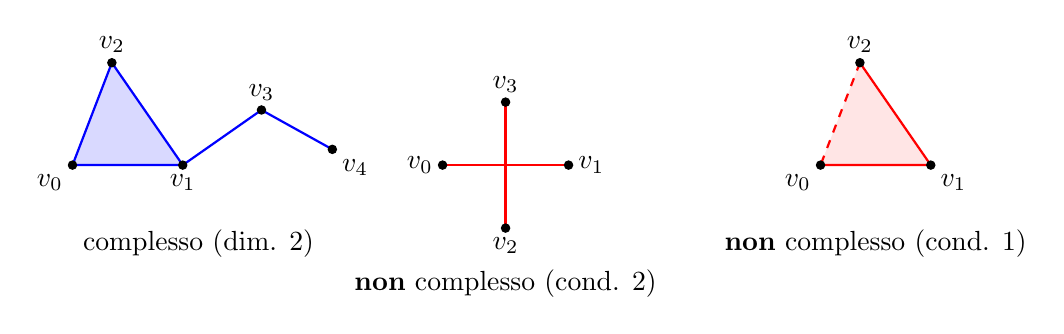
\begin{tikzpicture}[scale=1.0]
        % esempio 2
        \begin{scope}
            \fill[blue!15] (0,0) -- (1.4,0) -- (0.5,1.3) -- cycle;
            \draw[thick, blue] (0,0) -- (1.4,0) -- (0.5,1.3) -- cycle;
            \draw[thick, blue] (1.4,0) -- (2.4,0.7) -- (3.3,0.2);
            \foreach \p/\n/\d in {(0,0)/v_0/below left, (1.4,0)/v_1/below, (0.5,1.3)/v_2/above, (2.4,0.7)/v_3/above, (3.3,0.2)/v_4/below right}
                \filldraw \p circle (1.5pt) node[\d] {$\n$};
            \node at (1.6,-1.0) {complesso (dim. 2)};
        \end{scope}
        % controesempio 1
        \begin{scope}[shift={(5.5,0)}]
            \draw[thick, red] (-0.8,0) -- (0.8,0); \draw[thick, red] (0,-0.8) -- (0,0.8);
            \foreach \p/\n/\d in {(-0.8,0)/v_0/left, (0.8,0)/v_1/right, (0,-0.8)/v_2/below, (0,0.8)/v_3/above}
                \filldraw \p circle (1.5pt) node[\d] {$\n$};
            \node at (0,-1.5) {\textbf{non} complesso (cond. 2)};
        \end{scope}
        % controesempio 2
        \begin{scope}[shift={(9.5,0)}]
            \fill[red!10] (0,0) -- (1.4,0) -- (0.5,1.3) -- cycle;
            \draw[thick, red] (0,0) -- (1.4,0) -- (0.5,1.3);
            \draw[thick, red, dashed] (0.5,1.3) -- (0,0);
            \foreach \p/\n/\d in {(0,0)/v_0/below left, (1.4,0)/v_1/below right, (0.5,1.3)/v_2/above}
                \filldraw \p circle (1.5pt) node[\d] {$\n$};
            \node at (0.7,-1.0) {\textbf{non} complesso (cond. 1)};
        \end{scope}
    \end{tikzpicture}
    \caption{Un complesso simpliciale e due controesempi.}
\end{figure}


% ======== NUOVO (pp. 131-132) ========
\begin{ejemplo}[Altri esempi, continuazione]
\begin{enumerate}
    \item[7)] Nel caso del controesempio 1 (due segmenti che si incrociano) si ottiene un complesso simpliciale con lo stesso sostegno aggiungendo il punto di intersezione $v_4$ come nuovo vertice e dividendo i due segmenti:
    \[
    K = \{ (v_0), \dots, (v_4), (v_0, v_4), (v_1, v_4), (v_2, v_4), (v_3, v_4) \}.
    \]
    Invece, nel controesempio 2 (il triangolo senza un lato) \textbf{non esiste alcun complesso simpliciale con quel sostegno}: infatti il sostegno di un complesso simpliciale \`e unione di simplessi \emph{chiusi} (proposizione seguente), quindi \`e un insieme chiuso, mentre ``triangolo meno un lato aperto'' non \`e chiuso.
    \item[8)] Un triangolo pieno $[v_0, v_1, v_2]$ bucato trasversalmente da un segmento $(v_3, v_4)$ ha $(v_0, v_1, v_2) \cap (v_3, v_4) \neq \varnothing$, quindi non \`e un complesso simpliciale. Ne \`e il sostegno il complesso che si ottiene aggiungendo il punto di intersezione $v_5$ come vertice, suddividendo il triangolo in tre triangoli e il segmento in due:
    \begin{align*}
    K = \{ & (v_0), \dots, (v_5),\ (v_0,v_1), (v_0,v_2), (v_1,v_2), (v_0,v_5), (v_1,v_5), (v_2,v_5), (v_3,v_5), (v_4,v_5), \\
    & (v_0,v_1,v_5), (v_1,v_2,v_5), (v_0,v_2,v_5) \}.
    \end{align*}
    \item[9)] Ogni poligono \`e il sostegno di un complesso simpliciale (si triangola); di conseguenza ogni poliedro \`e il sostegno di un complesso simpliciale.
\end{enumerate}
\end{ejemplo}

\begin{figure}[H]
    \centering
    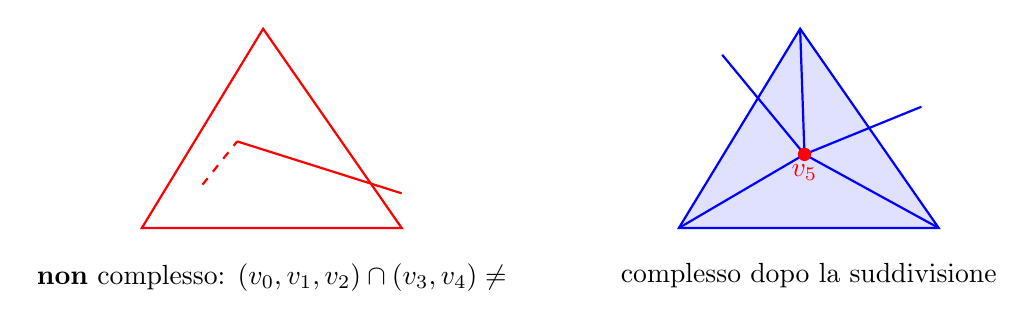
\begin{tikzpicture}[scale=1.1]
        % esempio 7: triangolo trafitto
        \begin{scope}
            \draw[thick, red] (0,0) -- (3,0) -- (1.4,2.3) -- cycle;
            \draw[thick, red] (1.1,1.0) -- (3.0,0.4);
            \draw[thick, red, dashed] (0.7,0.5) -- (1.1,1.0);
            \node[below] at (1.5,-0.3) {\textbf{non} complesso: $(v_0,v_1,v_2)\cap(v_3,v_4)\neq\varnothing$};
        \end{scope}
        \begin{scope}[shift={(6.2,0)}]
            \fill[blue!12] (0,0) -- (3,0) -- (1.4,2.3) -- cycle;
            \draw[thick, blue] (0,0) -- (3,0) -- (1.4,2.3) -- cycle;
            \coordinate (v5) at (1.45,0.85);
            \draw[thick, blue] (v5) -- (0,0); \draw[thick, blue] (v5) -- (3,0); \draw[thick, blue] (v5) -- (1.4,2.3);
            \draw[thick, blue] (v5) -- (0.5,2.0); \draw[thick, blue] (v5) -- (2.8,1.4);
            \filldraw[red] (v5) circle (2pt) node[below] {$v_5$};
            \node[below] at (1.5,-0.3) {complesso dopo la suddivisione};
        \end{scope}
    \end{tikzpicture}
    \caption{Per rendere ``simpliciale'' una configurazione in cui i simplessi si intersecano nel loro interno, si aggiunge il punto di intersezione come nuovo vertice e si suddivide.}
\end{figure}

\begin{prop}
Se $K$ \`e un complesso simpliciale, allora
\[
|K| = \bigcup_{(s) \in K} [s].
\]
In particolare $|K|$ \`e un sottoinsieme \textbf{chiuso} (e compatto) di $\mathbb{R}^n$, essendo unione finita di simplessi chiusi (che sono compatti).
\end{prop}
\begin{proof}
``$\subseteq$'': $|K| = \bigcup_{(s) \in K} (s) \subseteq \bigcup_{(s) \in K} [s]$, perch\'e $(s) \subseteq [s]$.
``$\supseteq$'': per ogni $(s) \in K$, $[s]$ \`e l'unione delle facce aperte $(s')$ di $(s)$ (esercizio precedente), che per la condizione 1) appartengono a $K$; dunque $[s] = \bigcup (s') \subseteq |K|$\hfill$\square$
\end{proof}

\begin{definicion}[$n$-scheletro]
Sia $K$ un complesso simpliciale, $m = \dim K$ e $n \in \{0, \dots, m\}$. Si chiama \textbf{$n$-scheletro} di $K$ il complesso simpliciale
\[
K^n = \{ (s) \in K \mid \dim (s) \leqslant n \}.
\]
\end{definicion}

\begin{observacion}
\begin{enumerate}
    \item $\dim K^n = n$.
    \item $K^m = K$.
    \item $K^0$ \`e l'insieme dei \textbf{vertici} di $K$.
\end{enumerate}
\end{observacion}

\begin{intuizione}
L'$n$-scheletro conserva tutti i simplessi di dimensione al pi\`u $n$ e ``butta via'' quelli pi\`u grandi: per un tetraedro pieno, $K^0$ sono i 4 vertici, $K^1$ lo scheletro dei 6 spigoli, $K^2$ la superficie (4 facce) e $K^3$ tutto il tetraedro. (\`E ancora un complesso simpliciale perch\'e le facce di un simplesso hanno dimensione minore.)
\end{intuizione}


% ======== NUOVO (pp. 133-134) ========
\begin{ejemplo}[Scheletri]
\begin{enumerate}
    \item Sia $K$ la decomposizione simpliciale del tetraedro $[v_0, v_1, v_2, v_3]$. Allora
    \begin{align*}
    K^0 &= \{ (v_0), (v_1), (v_2), (v_3) \}, \\
    K^1 &= K^0 \cup \{ (v_0,v_1), (v_0,v_2), (v_0,v_3), (v_1,v_2), (v_1,v_3), (v_2,v_3) \}, \\
    K^2 &= K^1 \cup \{ (v_0,v_1,v_2), (v_0,v_1,v_3), (v_0,v_2,v_3), (v_1,v_2,v_3) \}, \\
    K^3 &= K.
    \end{align*}
    \item Sia $K$ una triangolazione di un quadrato (con un vertice al centro e otto triangoli): $K^0$ sono i 9 vertici, $K^1$ \`e il grafo formato dai vertici e dagli spigoli, e $K = K^2$.
\end{enumerate}
\end{ejemplo}

\begin{figure}[H]
    \centering
    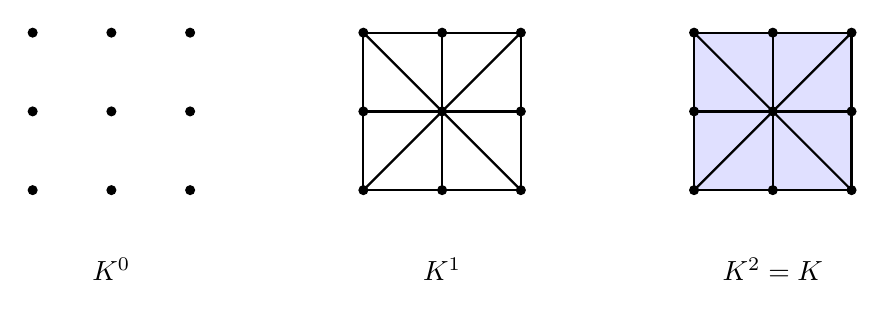
\begin{tikzpicture}[scale=1.0]
        \foreach \s/\name in {0/{$K^0$},4.2/{$K^1$},8.4/{$K^2 = K$}} {
            \begin{scope}[shift={(\s,0)}]
                \node at (1,-1.0) {\name};
            \end{scope}
        }
        % K^0
        \foreach \x in {0,1,2} \foreach \y in {0,1,2} { \filldraw (\x*1.0,\y*1.0) circle (1.6pt); }
        % K^1
        \begin{scope}[shift={(4.2,0)}]
            \draw[thick] (0,0) rectangle (2,2);
            \draw[thick] (1,0) -- (1,2); \draw[thick] (0,1) -- (2,1);
            \draw[thick] (0,0) -- (2,2); \draw[thick] (0,2) -- (2,0);
            \foreach \x in {0,1,2} \foreach \y in {0,1,2} { \filldraw (\x*1.0,\y*1.0) circle (1.6pt); }
        \end{scope}
        % K^2
        \begin{scope}[shift={(8.4,0)}]
            \fill[blue!12] (0,0) rectangle (2,2);
            \draw[thick] (0,0) rectangle (2,2);
            \draw[thick] (1,0) -- (1,2); \draw[thick] (0,1) -- (2,1);
            \draw[thick] (0,0) -- (2,2); \draw[thick] (0,2) -- (2,0);
            \foreach \x in {0,1,2} \foreach \y in {0,1,2} { \filldraw (\x*1.0,\y*1.0) circle (1.6pt); }
        \end{scope}
    \end{tikzpicture}
    \caption{Gli scheletri di una triangolazione del quadrato: vertici, grafo, e il complesso completo.}
\end{figure}

\begin{definicion}[Suddivisione]
Siano $K, K^*$ complessi simpliciali. Si dice che $K^*$ \`e una \textbf{suddivisione} di $K$ se $|K| = |K^*|$ e per ogni $(s) \in K^*$ esiste $(s') \in K$ tale che $(s) \subseteq (s')$.
\end{definicion}

\begin{intuizione}
$K^*$ ha lo stesso sostegno di $K$, ma i suoi simplessi sono ``pi\`u piccoli'': ciascun simplesso di $K^*$ sta dentro un simplesso di $K$. \`E una triangolazione pi\`u fine della stessa figura.
\end{intuizione}

\begin{ejemplo}
\begin{enumerate}
    \item Sia $K = \{ (v_0), (v_1), (v_0, v_1) \}$ (un segmento). Allora, con $v_2 \in (v_0, v_1)$,
    \[ K^* = \{ (v_0), (v_1), (v_2), (v_0, v_2), (v_2, v_1) \} \]
    \`e una suddivisione di $K$. Se prendessimo un altro punto $v_3 \in (v_0, v_1)$, avremmo un'altra suddivisione
    \[ K' = \{ (v_0), (v_3), (v_1), (v_0, v_3), (v_3, v_1) \} \]
    di $K$, \textbf{non confrontabile} con $K^*$ (n\'e $K'$ \`e suddivisione di $K^*$, n\'e viceversa).
    \item Sia $K = \{ \text{vertici } v_0, v_1, v_2,\ \text{lati},\ \text{triangolo} \}$ (un triangolo pieno). Aggiungendo i punti medi dei lati $v_3, v_4, v_5$ e dividendo in $4$ triangoli si ottiene una suddivisione $K^*$ di $K$; dividendo invece il triangolo in due con il segmento $(v_2, v_3)$, dove $v_3 \in (v_0, v_1)$, si ottiene un'altra suddivisione $K'$ di $K$, non confrontabile con $K^*$.
\end{enumerate}
\end{ejemplo}

\begin{figure}[H]
    \centering
    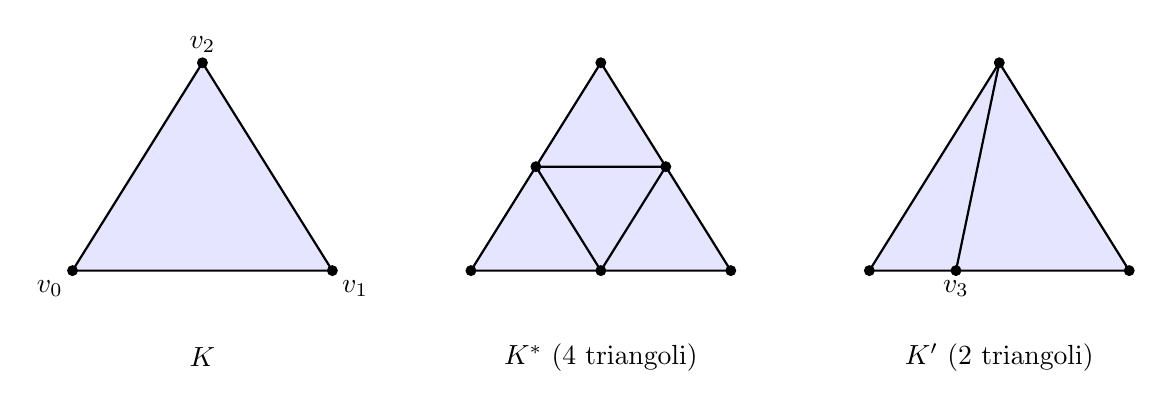
\begin{tikzpicture}[scale=1.1]
        \begin{scope}
            \fill[blue!10] (0,0) -- (3,0) -- (1.5,2.4) -- cycle;
            \draw[thick] (0,0) -- (3,0) -- (1.5,2.4) -- cycle;
            \filldraw (0,0) circle (1.6pt) node[below left] {$v_0$};
            \filldraw (3,0) circle (1.6pt) node[below right] {$v_1$};
            \filldraw (1.5,2.4) circle (1.6pt) node[above] {$v_2$};
            \node at (1.5,-1.0) {$K$};
        \end{scope}
        \begin{scope}[shift={(4.6,0)}]
            \fill[blue!10] (0,0) -- (3,0) -- (1.5,2.4) -- cycle;
            \draw[thick] (0,0) -- (3,0) -- (1.5,2.4) -- cycle;
            \draw[thick] (1.5,0) -- (0.75,1.2) -- (2.25,1.2) -- cycle;
            \foreach \p in {(0,0),(3,0),(1.5,2.4),(1.5,0),(0.75,1.2),(2.25,1.2)} \filldraw \p circle (1.6pt);
            \node at (1.5,-1.0) {$K^*$ (4 triangoli)};
        \end{scope}
        \begin{scope}[shift={(9.2,0)}]
            \fill[blue!10] (0,0) -- (3,0) -- (1.5,2.4) -- cycle;
            \draw[thick] (0,0) -- (3,0) -- (1.5,2.4) -- cycle;
            \draw[thick] (1.0,0) -- (1.5,2.4);
            \foreach \p in {(0,0),(3,0),(1.5,2.4),(1.0,0)} \filldraw \p circle (1.6pt);
            \node[below] at (1.0,0) {$v_3$};
            \node at (1.5,-1.0) {$K'$ (2 triangoli)};
        \end{scope}
    \end{tikzpicture}
    \caption{Due suddivisioni diverse e non confrontabili dello stesso triangolo $K$.}
\end{figure}


% ======== NUOVO (pp. 135-140) ========
\section{La suddivisione baricentrica}

\begin{definicion}[Ordine parziale in un complesso]
Sia $K$ un complesso simpliciale. Introduciamo in $K$ una relazione d'ordine parziale: per ogni $(s), (s') \in K$,
\[
(s) \leqslant (s') \iff (s) \subseteq [s'],
\]
cio\`e $(s)$ \`e una faccia aperta di $[s']$. \`E riflessiva, transitiva e antisimmetrica: se $(s) \leqslant (s')$ e $(s') \leqslant (s)$ allora $(s) \subseteq (s') \subseteq (s)$, cio\`e $(s) = (s')$. Due simplessi possono per\`o non essere confrontabili: ad esempio due vertici distinti.
\end{definicion}

Per ogni $(s) \in K$ indichiamo con $b(s)$ il \textbf{baricentro} di $(s)$.

\begin{teo}[Prima suddivisione baricentrica]
Dato un complesso simpliciale $K$ con $m = \dim K$, l'insieme
\[
K^{(1)} = \Big\{ \big( b(s_0), \dots, b(s_p) \big) \;\Big|\; p = 0, \dots, m,\ (s_0), \dots, (s_p) \in K,\ (s_i) < (s_{i+1})\ \forall i \Big\}
\]
(catene \emph{strettamente} crescenti di simplessi di $K$) \`e una suddivisione di $K$, detta \textbf{prima suddivisione baricentrica} di $K$. Si pone $K^{(2)} = (K^{(1)})^{(1)}, \dots, K^{(q)} = (K^{(q-1)})^{(1)}$.
\end{teo}

\begin{intuizione}
Per ottenere $K^{(1)}$ si mette un nuovo vertice nel baricentro di \emph{ogni} simplesso di $K$ (anche degli spigoli e dei triangoli) e poi si ``congiungono'' i baricentri ordinati per inclusione: baricentro di un vertice $\to$ baricentro di uno spigolo che lo contiene $\to$ baricentro di un triangolo che contiene lo spigolo $\to \dots$
\end{intuizione}

\begin{ejemplo}
\begin{enumerate}
    \item \textbf{Segmento.} $K = \{ (v_0), (v_1), (v_0, v_1) \}$. Il baricentro di $(v_0, v_1)$ \`e il punto medio $b$. Allora
    \[
    K^{(1)} = \{ (v_0), (v_1), (b), (v_0, b), (b, v_1) \}
    \]
    e, iterando, $(K^{(1)})^{(1)} = \{ (v_0), (v_1), (b), (b_1), (b_2), (v_0, b_1), (b_1, b), (b, b_2), (b_2, v_1) \}$, dove $b_1, b_2$ sono i punti medi di $(v_0, b)$ e $(b, v_1)$: il segmento viene diviso in $4$ parti uguali.
    \item \textbf{Triangolo.} Se $K$ \`e la decomposizione di un triangolo $[v_0, v_1, v_2]$, $K^{(1)}$ ha $7$ vertici ($3$ vertici, $3$ punti medi dei lati e il baricentro $b$ del triangolo) e $6$ triangoli: ciascuno ha vertici $\{$vertice, punto medio di un lato uscente da quel vertice, baricentro $b\}$.
\end{enumerate}
\end{ejemplo}

\begin{figure}[H]
    \centering
    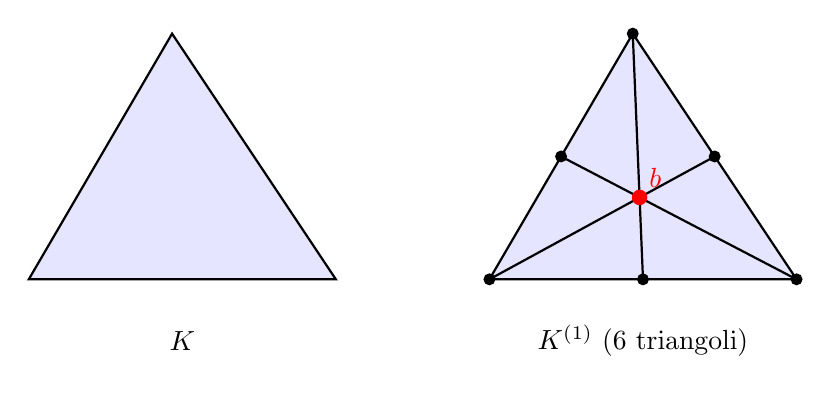
\begin{tikzpicture}[scale=1.3]
        \begin{scope}
            \fill[blue!10] (0,0) -- (3,0) -- (1.4,2.4) -- cycle;
            \draw[thick] (0,0) -- (3,0) -- (1.4,2.4) -- cycle;
            \node at (1.5,-0.6) {$K$};
        \end{scope}
        \begin{scope}[shift={(4.5,0)}]
            \coordinate (A) at (0,0); \coordinate (B) at (3,0); \coordinate (C) at (1.4,2.4);
            \coordinate (mAB) at (1.5,0); \coordinate (mBC) at (2.2,1.2); \coordinate (mAC) at (0.7,1.2);
            \coordinate (G) at (1.4667,0.8);
            \fill[blue!10] (A) -- (B) -- (C) -- cycle;
            \draw[thick] (A) -- (B) -- (C) -- cycle;
            \draw[thick] (A) -- (mBC); \draw[thick] (B) -- (mAC); \draw[thick] (C) -- (mAB);
            \foreach \p in {A,B,C,mAB,mBC,mAC} \filldraw (\p) circle (1.5pt);
            \filldraw[red] (G) circle (2pt) node[above right] {$b$};
            \node at (1.5,-0.6) {$K^{(1)}$ (6 triangoli)};
        \end{scope}
    \end{tikzpicture}
    \caption{La prima suddivisione baricentrica di un triangolo: le tre mediane lo dividono in $6$ triangoli.}
\end{figure}

\begin{prop}
Sia $[s] = [v_0, \dots, v_k]$ un $k$-simplesso. Allora:
\begin{enumerate}
    \item[(a)] per ogni $u, v \in [s]$: $d(u,v) \leqslant \max_{i,j = 0, \dots, k} d(v_i, v_j)$;
    \item[(b)] $\operatorname{diam}[s] = \max_{i,j = 0, \dots, k} d(v_i, v_j)$.
\end{enumerate}
In parole: il diametro di un simplesso \`e la lunghezza del suo spigolo pi\`u lungo.
\end{prop}
\begin{proof}
(a) Siano $u, v \in [s]$, $v = \sum_i t_i v_i$ con $t_i \geqslant 0$, $\sum t_i = 1$. Allora
\[
\begin{aligned}
d(u,v) = \|u - v\| &= \Big\| \Big(\sum_i t_i\Big) u - \sum_i t_i v_i \Big\| = \Big\| \sum_i t_i (u - v_i) \Big\| \\
&\leqslant \sum_i t_i \|u - v_i\| \leqslant \max_\delta \|u - v_\delta\| = \max_\delta d(u, v_\delta).
\end{aligned}
\]
Ora, scrivendo $u = \sum_j a_j v_j$ con $a_j \geqslant 0$, $\sum a_j = 1$, per ogni $\delta$:
\[
d(u, v_\delta) = \Big\| \sum_j a_j v_j - \Big(\sum_j a_j\Big) v_\delta \Big\| = \Big\| \sum_j a_j (v_j - v_\delta) \Big\| \leqslant \sum_j a_j \|v_j - v_\delta\| \leqslant \max_j d(v_j, v_\delta).
\]
Quindi $d(u, v) \leqslant \max_\delta d(u, v_\delta) \leqslant \max_{j, \delta} d(v_j, v_\delta)$.

(b) Per (a), $\operatorname{diam}[s] = \sup_{u,v \in [s]} d(u,v) \leqslant \max_{i,j} d(v_i, v_j)$; d'altra parte i vertici stanno in $[s]$, quindi $\max_{i,j} d(v_i, v_j) \leqslant \operatorname{diam}[s]$\hfill$\square$
\end{proof}

\begin{definicion}[Maglia]
Sia $K$ un complesso simpliciale. Si chiama \textbf{maglia} di $K$ il numero
\[
\operatorname{maglia}(K) = \max_{(s) \in K} \operatorname{diam}[s].
\]
\end{definicion}

\begin{teo}
Sia $K$ un complesso simpliciale, $m = \dim K$ e $n \in \mathbb{N}$. Allora
\[
0 \leqslant \operatorname{maglia}\big(K^{(n)}\big) \leqslant \left( \frac{m}{m+1} \right)^{n} \operatorname{maglia}(K) \ \ \Big( \leqslant \frac{m}{m+n} \operatorname{maglia}(K) \Big).
\]
\end{teo}

\begin{observacion}
Negli appunti la stima \`e scritta nella forma $\frac{m}{m+n}\operatorname{maglia}(K)$ (``senza dimostrazione''). Questa forma \`e vera, ma segue dalla stima pi\`u forte $\big(\frac{m}{m+1}\big)^n$, perch\'e per la disuguaglianza di Bernoulli $\big(1 + \frac1m\big)^n \geqslant 1 + \frac nm = \frac{m+n}{m}$, cio\`e $\big(\frac{m}{m+1}\big)^n \leqslant \frac{m}{m+n}$. Qui si dimostra il caso $n=1$ (da cui il caso generale per induzione, applicando il caso $n = 1$ a $K^{(n-1)}$, che ha ancora dimensione $m$).
\end{observacion}

\begin{proof}[Dimostrazione del caso $n=1$]
Un simplesso di $K^{(1)}$ ha vertici $b(s_0), \dots, b(s_p)$ con $(s_0) < \dots < (s_p)$ in $K$. Per la proposizione precedente il suo diametro \`e il massimo delle distanze tra due vertici, quindi basta stimare $d(b(s_i), b(s_j))$ con $i < j$. Poich\'e $b(s_i) \in [s_i] \subseteq [s_j]$, per il punto (a) della proposizione (la dimostrazione mostra $d(u, w) \leqslant \max_\delta d(u, w_\delta)$) si ha
\[
d(b(s_j), b(s_i)) \leqslant \max_{\delta} d(b(s_j), w_\delta),
\]
dove $w_0, \dots, w_q$ sono i vertici di $(s_j)$ ($q = \dim (s_j) \leqslant m$). Per ogni $\delta$,
\[
\|b(s_j) - w_\delta\| = \Big\| \frac{1}{q+1} \sum_{l} (w_l - w_\delta) \Big\| \leqslant \frac{q}{q+1} \max_l \|w_l - w_\delta\| \leqslant \frac{q}{q+1} \operatorname{diam}[s_j] \leqslant \frac{m}{m+1} \operatorname{maglia}(K),
\]
(il termine con $l = \delta$ \`e nullo, rimangono $q$ addendi; e $\frac{q}{q+1} \leqslant \frac{m}{m+1}$ perch\'e $q \leqslant m$). Dunque $\operatorname{maglia}(K^{(1)}) \leqslant \frac{m}{m+1} \operatorname{maglia}(K)$\hfill$\square$
\end{proof}

\begin{coro}
$\displaystyle \lim_{n \to +\infty} \operatorname{maglia}\big(K^{(n)}\big) = 0$.
\end{coro}

\begin{intuizione}
Suddividendo baricentricamente un numero sufficiente di volte, \emph{tutti} i simplessi diventano piccoli quanto si vuole, pur mantenendo lo stesso sostegno. Questo \`e lo strumento che servir\`a per mostrare che l'omologia simpliciale non dipende dalla triangolazione scelta.
\end{intuizione}

\section{Propriet\`a topologiche dei complessi simpliciali}

Sia $[s] = [v_0, \dots, v_k]$ un $k$-simplesso in $\mathbb{R}^n$ e $\Pi$ il $k$-piano da esso generato, cos\`i che $[s] \subseteq \Pi$. Per la proposizione sulle trasformazioni affini esiste una trasformazione affine $f: \mathbb{R}^n \to \mathbb{R}^n$ con $f(\Pi) = \mathcal{L}(e_1, \dots, e_k)$, dove $\{e_1, \dots, e_n\}$ \`e la base canonica. Osserviamo che una trasformazione affine \`e un omeomorfismo (composizione di una traslazione e di un isomorfismo lineare), quindi $f([s]) \subseteq \mathcal{L}(e_1, \dots, e_k)$ \`e omeomorfo a $[s]$.

Poich\'e $f(v_0) = \bar{0}$ e $f(v_i) = e_i$ ($i = 1, \dots, k$) (la parte lineare di $f$ manda $v_i - v_0$ in $e_i$), e $f$ conserva le combinazioni affini, per $v = \sum_i t_i v_i \in [s]$ si ha $f(v) = \sum_{i=1}^k t_i e_i$ con $t_i \geqslant 0$ e $t_1 + \dots + t_k = 1 - t_0 \leqslant 1$. Quindi
\[
f([s]) = \Big\{ x \in \mathbb{R}^k \;\Big|\; x = \sum_{i=1}^k t_i e_i,\ t_i \geqslant 0,\ \sum_{i=1}^k t_i \leqslant 1 \Big\} = \Delta^k,
\]
il \textbf{simplesso standard} di $\mathbb{R}^k$ (l'insieme dei punti di $\mathcal{L}(e_1, \dots, e_k) \cong \mathbb{R}^k$ con coordinate $\geqslant 0$ e somma $\leqslant 1$). Per $k = 1$: $\mathbb{R} = \mathcal{L}(e_1)$ e $[\bar{0}, e_1] = \{ t e_1 \mid 0 \leqslant t \leqslant 1 \}$.

\begin{prop}
Ogni $k$-simplesso chiuso $[s] \subset \mathbb{R}^n$ \`e omeomorfo al simplesso standard $\Delta^k \subset \mathbb{R}^k$ (e in particolare \`e compatto e connesso per archi, perch\'e $\Delta^k$ \`e chiuso e limitato e convesso).
\end{prop}


% ======== NUOVO (pp. 141-144) ========
Per $k=2$ si ha $\mathbb{R}^2 = \mathcal{L}(e_1, e_2)$ e
\[
[\bar{0}, e_1, e_2] = \{ v \in \mathbb{R}^2 \mid v = t_1 e_1 + t_2 e_2,\ t_1, t_2 \geqslant 0,\ t_1 + t_2 \leqslant 1 \},
\]
il triangolo di vertici $(0,0), (1,0), (0,1)$; per $k = 3$, $[\bar{0}, e_1, e_2, e_3]$ \`e il tetraedro con $t_1, t_2, t_3 \geqslant 0$ e $t_1 + t_2 + t_3 \leqslant 1$.

\begin{figure}[H]
    \centering
    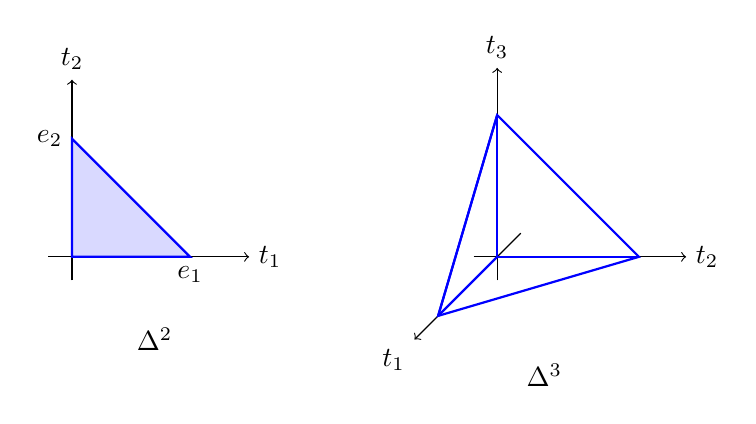
\begin{tikzpicture}[scale=1.5]
        \begin{scope}
            \draw[->] (-0.2,0) -- (1.5,0) node[right] {$t_1$};
            \draw[->] (0,-0.2) -- (0,1.5) node[above] {$t_2$};
            \fill[blue!15] (0,0) -- (1,0) -- (0,1) -- cycle;
            \draw[thick, blue] (0,0) -- (1,0) -- (0,1) -- cycle;
            \node[below] at (1,0) {$e_1$}; \node[left] at (0,1) {$e_2$};
            \node at (0.7,-0.7) {$\Delta^2$};
        \end{scope}
        \begin{scope}[shift={(3.6,0)}]
            \draw[->] (-0.2,0) -- (1.6,0) node[right] {$t_2$};
            \draw[->] (0,-0.2) -- (0,1.6) node[above] {$t_3$};
            \draw[->] (0.2,0.2) -- (-0.7,-0.7) node[below left] {$t_1$};
            \draw[thick, blue] (-0.5,-0.5) -- (1.2,0) -- (0,1.2) -- cycle;
            \draw[thick, blue] (0,0) -- (-0.5,-0.5); \draw[thick, blue] (0,0) -- (1.2,0); \draw[thick, blue] (0,0) -- (0,1.2);
            \draw[thick, blue] (-0.5,-0.5) -- (0,1.2);
            \node at (0.4,-1.0) {$\Delta^3$};
        \end{scope}
    \end{tikzpicture}
    \caption{I simplessi standard $\Delta^2 \subset \mathbb{R}^2$ e $\Delta^3 \subset \mathbb{R}^3$.}
\end{figure}

\begin{observacion}[Conseguenza]
$f([s])$ (e quindi anche $[s]$) \`e un sottoinsieme chiuso e limitato di $\mathbb{R}^n$, dunque \textbf{compatto}.
\end{observacion}

\begin{prop}
Sia $K$ un complesso simpliciale. Allora:
\begin{enumerate}
    \item[a)] $|K|$ \`e compatto;
    \item[b)] $\{ [s] \}_{(s) \in K}$ \`e un ricoprimento \textbf{finito} di \textbf{chiusi} di $|K|$.
\end{enumerate}
\end{prop}
\begin{proof}
Si ha $|K| = \bigcup_{(s) \in K} [s]$, unione finita di compatti (quindi compatta e chiusa) e ciascun $[s]$ \`e chiuso\hfill$\square$
\end{proof}

\begin{prop}
Per ogni spazio topologico $X$ e ogni applicazione $f: |K| \to X$:
\[
f \text{ \`e continua} \iff f|_{[s]} \text{ \`e continua per ogni } (s) \in K.
\]
\end{prop}
\begin{proof}
($\Rightarrow$) \`E banale (restrizione di una continua). ($\Leftarrow$) Segue dal punto b) della proposizione precedente e dal Lemma di Incollamento (ricoprimento finito di chiusi)\hfill$\square$
\end{proof}

\begin{intuizione}
Per controllare la continuit\`a di una funzione su un complesso basta controllarla simplesso per simplesso: \`e il principio che permette di definire applicazioni ``a pezzi'' (lineari su ciascun simplesso) e di ottenere automaticamente applicazioni continue.
\end{intuizione}

\section{Coordinate baricentriche di un complesso}

Siano $K$ un complesso simpliciale e $v \in K^0$ un vertice. Sia $w \in |K| = \bigsqcup_{(s) \in K} (s)$. Allora esiste un \textbf{unico} $(s) \in K$ con $w \in (s)$. Se $(s) = (v_0, \dots, v_k)$, allora $w = \sum_{i=0}^k t_i v_i$ con $t_i > 0$ per ogni $i$ e $\sum_{i=0}^k t_i = 1$. Poniamo
\[
t_v(w) = \begin{cases} 0 & \text{se } v \neq v_i \ \ \forall i = 0, \dots, k, \\ t_i & \text{se } v = v_i. \end{cases}
\]

\begin{definicion}
L'applicazione $t_v: |K| \to \mathbb{R}$, $w \mapsto t_v(w)$ si chiama \textbf{(funzione) coordinata baricentrica} di $K$ rispetto al vertice $v$.
\end{definicion}

\begin{prop}
$t_v: |K| \to \mathbb{R}$ \`e continua.
\end{prop}
\begin{proof}
Per la proposizione precedente basta verificare che $t_v|_{[s]}$ sia continua per ogni $(s) \in K$. Ora, per ogni $(s) \in K$:
\begin{itemize}
    \item se $v$ \textbf{non} \`e un vertice di $[s]$, allora $t_v|_{[s]} \equiv 0$ (ogni punto di $[s]$ sta in una faccia aperta i cui vertici sono vertici di $[s]$): \`e costante, dunque continua;
    \item se $v = v_i$ \`e un vertice di $[s]$, allora $t_v|_{[s]}$ \`e la $i$-esima coordinata baricentrica di $[s]$, che \`e continua perch\'e, via l'omeomorfismo affine $f: [s] \to \Delta^k$, \`e (a meno di un'identificazione) una funzione coordinata (lineare) su $\Delta^k$ (con $t_0 = 1 - t_1 - \dots - t_k$)\hfill$\square$
\end{itemize}
\end{proof}

\begin{ejemplo}
Sia $K$ la decomposizione del triangolo $[v_0, v_1, v_2]$.
\begin{itemize}
    \item Se $w \in (v_1, v_2)$, allora esiste un unico $t \in\, ]0,1[$ con $w = (1-t)v_1 + tv_2$, quindi $t_{v_0}(w) = 0$, $t_{v_1}(w) = 1-t$, $t_{v_2}(w) = t$.
    \item Per il vertice $v_0 \in (v_0) \in K$ si ha $v_0 = 1 \cdot v_0$, quindi $t_{v_0}(v_0) = 1$, $t_{v_1}(v_0) = 0$, $t_{v_2}(v_0) = 0$.
    \item Se $x \in (v_0, v_1, v_2)$, allora $x = (1 - t_1 - t_2)v_0 + t_1 v_1 + t_2 v_2$, e dunque $t_{v_0}(x) = 1 - t_1 - t_2$, $t_{v_1}(x) = t_1$, $t_{v_2}(x) = t_2$.
\end{itemize}
In tutti i casi: $v_0 = \sum_{i=0}^2 t_{v_i}(v_0) v_i$, $w = \sum_{i=0}^2 t_{v_i}(w) v_i$, $x = \sum_{i=0}^2 t_{v_i}(x) v_i$.
\end{ejemplo}

\begin{prop}
Sia $K$ un complesso simpliciale. Allora per ogni $x \in |K|$
\[
x = \sum_{v \in K^0} t_v(x) \cdot v, \qquad \text{con } t_v(x) \geqslant 0 \ \ \forall v \in K^0 \quad \text{e} \quad \sum_{v \in K^0} t_v(x) = 1 .
\]
\end{prop}
\begin{proof}
Sia $x \in |K| = \bigsqcup_{(s) \in K} (s)$; esiste un unico $(s) = (v_0, \dots, v_k) \in K$ con $x \in (s)$, e $x = \sum_{i=0}^k t_i v_i$ con $t_i > 0$, $\sum t_i = 1$. Per definizione $t_{v_i}(x) = t_i$ e $t_v(x) = 0$ per ogni vertice $v \in K^0$ diverso da $v_0, \dots, v_k$. Quindi
\[
\sum_{v \in K^0} t_v(x)\, v = \underbrace{\sum_{v \notin \{v_0, \dots, v_k\}} t_v(x)\, v}_{=0} + \sum_{i=0}^k t_{v_i}(x)\, v_i = \sum_{i=0}^k t_i v_i = x,
\]
e analogamente $t_v(x) \geqslant 0$ per ogni $v$ e $\sum_{v \in K^0} t_v(x) = \sum_{i=0}^k t_i = 1$\hfill$\square$
\end{proof}

\begin{intuizione}
Le funzioni $t_v$, $v \in K^0$, forniscono un sistema di ``coordinate globali'' su $|K|$ (le \emph{coordinate baricentriche} di $K$): un punto di $|K|$ \`e determinato dai pesi $(t_v(x))_{v \in K^0}$, non nulli solo sui vertici dell'unico simplesso aperto che lo contiene.
\end{intuizione}


% ======== NUOVO (pp. 145-148) ========
\begin{lema}
Per ogni $x, y \in |K|$: $\ x = y \iff t_v(x) = t_v(y)$ per ogni $v \in K^0$.
\end{lema}
\begin{proof}
($\Rightarrow$) \`E banale. ($\Leftarrow$) Per la proposizione precedente $x = \sum_{v \in K^0} t_v(x)\, v = \sum_{v \in K^0} t_v(y)\, v = y$\hfill$\square$
\end{proof}

\begin{prop}
$|K|$ \`e uno spazio di Hausdorff ($T_2$).
\end{prop}
\begin{proof}
Siano $x, y \in |K|$, $x \neq y$. Per il lemma esiste $v \in K^0$ con $t_v(x) \neq t_v(y)$; senza perdita di generalit\`a $t_v(x) < t_v(y)$, e sia $r \in \mathbb{R}$ con $t_v(x) < r < t_v(y)$. Poich\'e $t_v$ \`e continua,
\[
A = t_v^{-1}\big(\,]-\infty, r[\,\big), \qquad B = t_v^{-1}\big(\,]r, +\infty[\,\big)
\]
sono aperti di $|K|$, con $x \in A$, $y \in B$ e $A \cap B = \varnothing$\hfill$\square$
\end{proof}

(Naturalmente $|K| \subset \mathbb{R}^n$ \`e Hausdorff anche perch\'e sottospazio di $\mathbb{R}^n$; la dimostrazione precedente \`e utile perch\'e usa solo le coordinate baricentriche.)

\begin{definicion}[Stella di un vertice]
Sia $K$ un complesso simpliciale e $v \in K^0$. Si chiama \textbf{stella} di $v$ l'insieme
\[
\operatorname{st}(v) = \bigcup_{\substack{(s) \in K \\ v \in [s]}} (s),
\]
cio\`e l'unione di tutti i simplessi aperti di $K$ che hanno $v$ come vertice.
\end{definicion}

\begin{intuizione}
La stella di $v$ \`e l'``intorno naturale'' di $v$ nel complesso: i punti che si raggiungono da $v$ muovendosi dentro i simplessi (aperti) che contengono $v$ come vertice, \emph{senza} le facce opposte a $v$.
\end{intuizione}

\begin{ejemplo}
\begin{enumerate}
    \item $K = \{ (v_0), (v_1), (v_0, v_1) \}$ (un segmento). Allora $\operatorname{st}(v_0) = (v_0) \cup (v_0, v_1) = [v_0, v_1] \setminus \{v_1\}$.
    \item $K$ = decomposizione del triangolo $[v_0, v_1, v_2]$. Allora
    \[
    \operatorname{st}(v_0) = (v_0) \cup (v_0, v_1) \cup (v_0, v_2) \cup (v_0, v_1, v_2) = [v_0, v_1, v_2] \setminus [v_1, v_2],
    \]
    cio\`e il triangolo privato del lato opposto a $v_0$.
    \item Sia $K$ formato da un triangolo pieno $[v_0, v_1, v_2]$ a cui sono attaccati in $v_1$ due spigoli $(v_1, v_3)$ e $(v_1, v_4)$, con $v_4$ vertice di un secondo triangolo pieno $[v_4, v_5, v_6]$. Allora $\operatorname{st}(v_0) = [v_0, v_1, v_2] \setminus [v_1, v_2]$; $\operatorname{st}(v_3) = (v_3) \cup (v_1, v_3) = [v_1, v_3] \setminus \{v_1\}$; e $\operatorname{st}(v_1)$ \`e l'unione di $(v_1)$, degli spigoli $(v_0,v_1)$, $(v_1,v_2)$, $(v_1, v_3)$, $(v_1, v_4)$ e del triangolo aperto $(v_0, v_1, v_2)$.
\end{enumerate}
\end{ejemplo}

\begin{figure}[H]
    \centering
    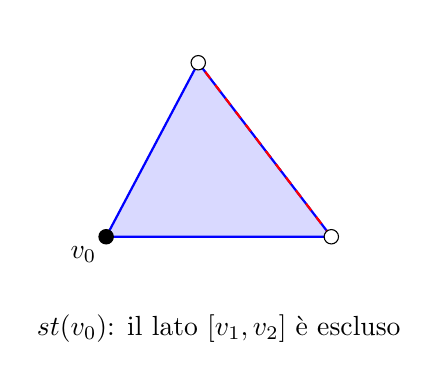
\begin{tikzpicture}[scale=1.3]
        \begin{scope}
            \fill[blue!15] (0,0) -- (2.2,0) -- (0.9,1.7) -- cycle;
            \draw[thick, blue] (0,0) -- (2.2,0) -- (0.9,1.7) -- cycle;
            \draw[thick, dashed, red] (2.2,0) -- (0.9,1.7);
            \filldraw (0,0) circle (2pt) node[below left] {$v_0$};
            \filldraw[white, draw=black] (2.2,0) circle (2pt) node[below right] {$v_1$};
            \filldraw[white, draw=black] (0.9,1.7) circle (2pt) node[above] {$v_2$};
            \node at (1.1,-0.9) {$\operatorname{st}(v_0)$: il lato $[v_1,v_2]$ \`e escluso};
        \end{scope}
    \end{tikzpicture}
    \caption{La stella di $v_0$ in un triangolo: tutto tranne il lato opposto (cerchi vuoti e tratteggio indicano punti esclusi).}
\end{figure}

\begin{prop}
Sia $K$ un complesso simpliciale e $v \in K^0$. Allora:
\begin{enumerate}
    \item[(1)] $\operatorname{st}(v)$ \`e un aperto di $|K|$;
    \item[(2)] se $v' \in K^0$ e $v' \in \operatorname{st}(v)$, allora $v' = v$ (la stella di $v$ contiene un solo vertice: $v$ stesso).
\end{enumerate}
\end{prop}
\begin{proof}
(1) Si ha $\operatorname{st}(v) = t_v^{-1}\big(\,]0, +\infty[\,\big)$: infatti $t_v(w) > 0$ se e solo se $v$ \`e un vertice dell'unico simplesso aperto $(s)$ che contiene $w$, cio\`e $w \in \operatorname{st}(v)$. Essendo $t_v$ continua, $\operatorname{st}(v)$ \`e aperto.

(2) Se $v' \in \operatorname{st}(v)$, esiste un unico $(s) \in K$ con $v' \in (s)$ e $v \in [s]$. Poich\'e $v'$ \`e un vertice, l'unico simplesso aperto che lo contiene \`e $(v')$, quindi $(s) = (v')$, e $v \in [s] = [v'] = \{v'\}$, cio\`e $v = v'$\hfill$\square$
\end{proof}

\begin{prop}
$\{ \operatorname{st}(v) \}_{v \in K^0}$ \`e un ricoprimento aperto e finito di $|K|$.
\end{prop}
\begin{proof}
Ogni $w \in |K|$ sta in un simplesso aperto $(s)$, che ha almeno un vertice $v$; allora $w \in \operatorname{st}(v)$. I $\operatorname{st}(v)$ sono aperti per la proposizione precedente e sono in numero finito perch\'e $K^0$ \`e finito\hfill$\square$
\end{proof}


% ======== NUOVO (pp. 147-152): Richiami sui gruppi abeliani, commutatori, simplessi orientati ========
\section{Richiami sui gruppi abeliani}

Sia $(G, +)$ un gruppo abeliano. Per ogni $x \in G$ e $k \in \mathbb{Z}$ poniamo
\[
kx = \begin{cases} \underbrace{x + \dots + x}_{k} & \text{se } k > 0, \\ 0 & \text{se } k = 0, \\ \underbrace{(-x) + \dots + (-x)}_{|k|} & \text{se } k < 0. \end{cases}
\]

\begin{definicion}[Generatori, indipendenza, base]
\begin{itemize}
    \item Una famiglia $(x_i)_{i \in I} \subseteq G$ si dice \textbf{insieme di generatori} per $G$ se per ogni $x \in G$ esistono $F \subseteq I$ finito, $F = \{j_1, \dots, j_n\}$, e $k_1, \dots, k_n \in \mathbb{Z}$ tali che $x = \sum_{i=1}^n k_i x_{j_i}$.
    \item $(x_i)_{i \in I}$ si dice \textbf{libero} (o linearmente indipendente) se per ogni $F \subseteq I$ finito, $F = \{j_1, \dots, j_n\}$, e per ogni $k_1, \dots, k_n \in \mathbb{Z}$: $\sum_{i=1}^n k_i x_{j_i} = 0 \implies k_i = 0$ per ogni $i = 1, \dots, n$.
    \item $(x_i)_{i \in I}$ si dice \textbf{base} di $G$ se \`e un sistema di generatori ed \`e libero. Un gruppo che ammette una base si dice \textbf{libero}.
    \item $(G, +)$ si dice \textbf{finitamente generato} se $G$ ammette un sistema di generatori finito.
\end{itemize}
Se $(G, +)$ \`e libero, tutte le sue basi hanno la stessa cardinalit\`a, che prende il nome di \textbf{rango} di $G$.
\end{definicion}

\begin{ejemplo}
$\mathbb{Z}^n$ \`e libero di rango $n$ (base canonica); $\mathbb{Z}_2$ \`e finitamente generato ma \emph{non} libero (l'elemento $1$ genera, ma $2 \cdot 1 = 0$ con $2 \neq 0$).
\end{ejemplo}

\begin{definicion}[Gruppo ciclico]
$(G, +)$ si dice \textbf{ciclico} se \`e generato da un unico elemento $x \in G$. A meno di isomorfismi: esiste un unico gruppo ciclico infinito, $\mathbb{Z}$, ed esiste un unico gruppo ciclico finito di ordine $n$, $\mathbb{Z}_n$, per ogni $n \in \mathbb{N}$, $n \geqslant 1$.
\end{definicion}

\begin{definicion}[Elemento di torsione]
Sia $(G, +)$ un gruppo abeliano. Un elemento $x \in G$ si dice \textbf{elemento di torsione} se esiste $k \in \mathbb{N}$, $k \geqslant 1$, tale che $kx = 0$.
\end{definicion}

\begin{prop}
L'insieme $\Gamma = \{ x \in G \mid x \text{ \`e di torsione} \}$ \`e un sottogruppo di $G$ (detto \textbf{sottogruppo di torsione}).
\end{prop}
\begin{proof}
Basta mostrare che per ogni $x, y \in \Gamma$ si ha $x - y \in \Gamma$. Se $kx = 0$ e $hy = 0$ con $k, h \geqslant 1$, allora $kh \geqslant 1$ e $kh(x - y) = h(kx) - k(hy) = h \cdot 0 - k \cdot 0 = 0$\hfill$\square$
\end{proof}

\begin{definicion}
Se $\Gamma$ \`e finito, la sua cardinalit\`a si chiama \textbf{ordine} di $\Gamma$. Se $\Gamma = \{0\}$, il gruppo $(G, +)$ si dice \textbf{privo di torsione}.
\end{definicion}

\begin{prop}[Propriet\`a]
\begin{enumerate}
    \item[a)] $G$ libero $\implies$ $G$ privo di torsione.
    \item[b)] Se $G$ \`e finitamente generato, allora $G$ privo di torsione $\implies$ $G$ libero. (Negli appunti questo punto compare scritto come la stessa implicazione del punto a); la forma corretta e standard \`e il viceversa, valido per i gruppi finitamente generati.)
    \item[c)] $G = G_1 \oplus G_2 \implies G/G_1 \cong G_2$.
    \item[d)] Se $G$ \`e finitamente generato e $H \leqslant G$, allora $G/H$ \`e finitamente generato.
\end{enumerate}
\end{prop}

\begin{teo}[Teorema fondamentale sui gruppi abeliani di tipo finito]
Sia $(G, +)$ un gruppo abeliano finitamente generato. Allora esiste un sottogruppo \textbf{libero} $G_0$ di $G$ tale che
\[
G = G_0 \oplus \Gamma ,
\]
dove $\Gamma$ \`e il sottogruppo di torsione. Si chiama \textbf{rango} di $G$ il rango di $G_0$. Inoltre $\Gamma$ \`e somma diretta di un numero finito $k$ di gruppi ciclici $\Gamma_1, \dots, \Gamma_k$ di ordini $t_1, \dots, t_k$ rispettivamente (nella forma standard, con $t_i > 1$ e $t_1 \mid t_2 \mid \dots \mid t_k$). In conclusione
\[
G \cong \mathbb{Z}^r \oplus \mathbb{Z}_{t_1} \oplus \dots \oplus \mathbb{Z}_{t_k}, \qquad r = \operatorname{rango}(G).
\]
\end{teo}
\begin{observacion}
Il testo del teorema nel PDF si interrompe a fine pagina dopo ``$\Gamma_1, \dots, \Gamma_k$ di ordine $t_1, \dots, t_k$ rispettivamente, con \dots''; qui \`e stata completata con l'enunciato standard (fattori invarianti).
\end{observacion}

\subsection{Commutatore e abelianizzato}

\begin{definicion}[Commutatore]
Sia $(G, \cdot)$ un gruppo e $a, b \in G$. L'elemento $[a, b] = a b a^{-1} b^{-1}$ si chiama \textbf{commutatore} di $a$ e $b$. Esso ``stima di quanto $a$ e $b$ siano lontani dal commutare'', perch\'e $[a,b] = e \iff ab = ba$. Si chiama \textbf{commutatore} di $G$ l'insieme $[G, G] = \{ [a,b] \mid a, b \in G \}$, e \textbf{derivato} di $G$ il sottogruppo $G'$ generato da $[G, G]$.
\end{definicion}

\begin{observacion}
\begin{enumerate}
    \item Ogni $x \in G'$ \`e il prodotto di un numero finito di commutatori (e dei loro inversi, che sono ancora commutatori: $[a,b]^{-1} = [b,a]$).
    \item $G'$ \`e un sottogruppo \textbf{normale} di $G$ (il coniugato di un commutatore \`e un commutatore: $g[a,b]g^{-1} = [gag^{-1}, gbg^{-1}]$).
    \item $G$ \`e abeliano $\iff$ $[G, G] = \{e\}$ (cio\`e $G' = \{e\}$).
\end{enumerate}
\end{observacion}

\begin{prop}
$G/G'$ \`e un gruppo abeliano, detto \textbf{abelianizzato} di $G$. Vale
\[
G' = \bigcap_{\substack{H \trianglelefteq G \\ G/H \text{ abeliano}}} H ,
\]
quindi $G/G'$ \`e il \textbf{pi\`u grande quoziente abeliano} di $G$.
\end{prop}
\begin{intuizione}
Abelianizzare significa ``far commutare'' tutto, cio\`e identificare $ab$ con $ba$. Ad esempio, l'abelianizzato del gruppo libero $F_2 = \langle a, b \rangle$ \`e $\mathbb{Z}^2$: \`e questo il motivo per cui, a differenza di $\Pi_1$, i gruppi di omologia che costruiremo sono sempre abeliani.
\end{intuizione}

\section{Simplessi orientati}

Sia $[s] = [v_0, \dots, v_k]$ un $k$-simplesso e siano $(i_0, \dots, i_k)$ e $(j_0, \dots, j_k)$ due permutazioni di $\{0, \dots, k\}$. Poniamo
\[
(i_0, \dots, i_k) \sim (j_0, \dots, j_k) \iff (j_0, \dots, j_k) \text{ \`e una permutazione \emph{pari} di } (i_0, \dots, i_k),
\]
cio\`e si ottiene da essa con un numero pari di trasposizioni. Se $P$ \`e l'insieme di tutte le permutazioni, allora per ogni $k \geqslant 1$ il quoziente $P/\!\sim$ ha esattamente \textbf{2 elementi} (le permutazioni pari e le dispari).

\begin{definicion}[Simplesso orientato]
Si chiama \textbf{$k$-simplesso orientato} e si indica con $\langle s \rangle = \langle v_{j_0}, \dots, v_{j_k} \rangle$ un $k$-simplesso $[s] = [v_0, \dots, v_k]$ munito di una classe fissata in $P/\!\sim$. Ciascun elemento di $P/\!\sim$ si chiama \textbf{orientazione} del $k$-simplesso.
\end{definicion}

Se $(i_0, \dots, i_k)$ \`e un'altra permutazione di $\{0, \dots, k\}$, allora
\[
\langle v_{i_0}, \dots, v_{i_k} \rangle = \begin{cases} \ \ \langle v_{j_0}, \dots, v_{j_k} \rangle & \text{se } (i_0, \dots, i_k) \sim (j_0, \dots, j_k), \\ -\langle v_{j_0}, \dots, v_{j_k} \rangle & \text{se } (i_0, \dots, i_k) \not\sim (j_0, \dots, j_k). \end{cases}
\]

\begin{intuizione}
Orientare un simplesso significa scegliere un ``verso di percorrenza'': per un segmento, quale estremo \`e l'inizio ($\langle v_0, v_1 \rangle = - \langle v_1, v_0 \rangle$); per un triangolo, il verso orario o antiorario ($\langle v_0, v_1, v_2 \rangle = \langle v_1, v_2, v_0 \rangle = - \langle v_1, v_0, v_2 \rangle$); per un tetraedro, la ``chiralit\`a'' (destra o sinistra). Scambiare due vertici inverte l'orientazione.
\end{intuizione}

\begin{figure}[H]
    \centering
    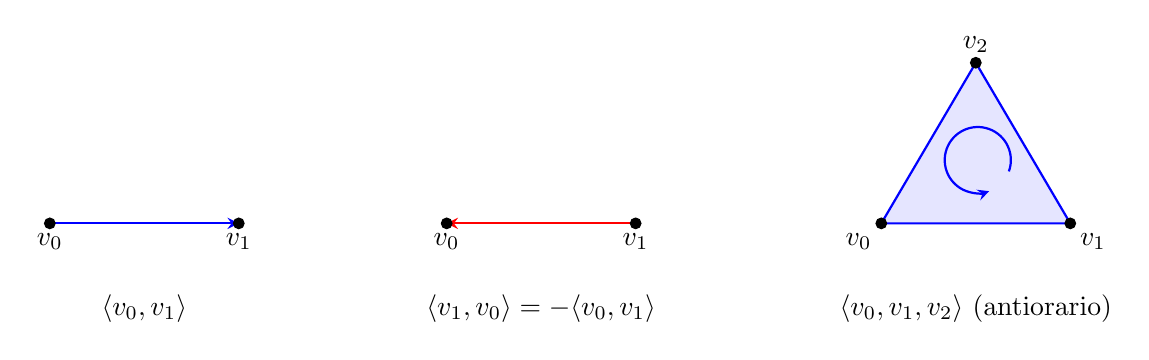
\begin{tikzpicture}[scale=1.2]
        \begin{scope}
            \draw[thick, ->, >=stealth, blue] (0,0) -- (2,0);
            \filldraw (0,0) circle (1.6pt) node[below] {$v_0$};
            \filldraw (2,0) circle (1.6pt) node[below] {$v_1$};
            \node at (1,-0.9) {$\langle v_0, v_1 \rangle$};
        \end{scope}
        \begin{scope}[shift={(4.2,0)}]
            \draw[thick, ->, >=stealth, red] (2,0) -- (0,0);
            \filldraw (0,0) circle (1.6pt) node[below] {$v_0$};
            \filldraw (2,0) circle (1.6pt) node[below] {$v_1$};
            \node at (1,-0.9) {$\langle v_1, v_0 \rangle = -\langle v_0, v_1 \rangle$};
        \end{scope}
        \begin{scope}[shift={(8.8,0)}]
            \fill[blue!10] (0,0) -- (2,0) -- (1,1.7) -- cycle;
            \draw[thick, blue] (0,0) -- (2,0) -- (1,1.7) -- cycle;
            \draw[->, >=stealth, thick, blue] (1.35,0.55) arc (-20:290:0.35);
            \filldraw (0,0) circle (1.6pt) node[below left] {$v_0$};
            \filldraw (2,0) circle (1.6pt) node[below right] {$v_1$};
            \filldraw (1,1.7) circle (1.6pt) node[above] {$v_2$};
            \node at (1,-0.9) {$\langle v_0, v_1, v_2 \rangle$ (antiorario)};
        \end{scope}
    \end{tikzpicture}
    \caption{Orientazione di un $1$-simplesso e di un $2$-simplesso.}
\end{figure}


% ======== NUOVO (pp. 153-156) ========
\begin{observacion}
Per ogni $k \geqslant 1$: $-\langle v_{j_0}, v_{j_1}, \dots, v_{j_k} \rangle = \langle v_{j_1}, v_{j_0}, \dots, v_{j_k} \rangle$ (scambiare due vertici \`e una permutazione dispari: inverte l'orientazione).
\end{observacion}

\begin{ejemplo}
\begin{enumerate}
    \item $k = 0$: $[v_0] = \{v_0\} = \langle v_0 \rangle$ ha un'unica orientazione naturale.
    \item $k = 1$: $[v_0, v_1] = \overline{v_0 v_1}$. Le permutazioni di $\{0,1\}$ sono $(0,1)$ e $(1,0)$ e $(0,1) \not\sim (1,0)$. Quindi ci sono due $1$-simplessi orientati: $\langle v_0, v_1 \rangle$ (percorso da $v_0$ a $v_1$) e $\langle v_1, v_0 \rangle = -\langle v_0, v_1 \rangle$ (percorso nel verso opposto).
    \item $k = 2$: a $[v_0, v_1, v_2]$ corrispondono i due $2$-simplessi orientati $\langle v_0, v_1, v_2 \rangle$ e $-\langle v_0, v_1, v_2 \rangle = \langle v_1, v_0, v_2 \rangle$ (i due versi di percorrenza del bordo del triangolo).
\end{enumerate}
In generale, un $k$-simplesso orientato $\langle s \rangle$ \`e il corrispondente $k$-simplesso chiuso in cui, avendo specificato un ordinamento dei vertici (e quindi dei $k$ vettori linearmente indipendenti $v_{j_1} - v_{j_0}, \dots, v_{j_k} - v_{j_0}$), \`e specificata un'\textbf{orientazione del $k$-piano} $\Pi \supseteq [s]$.
\end{ejemplo}

\section{Il gruppo delle $p$-catene}

Sia $K$ un complesso simpliciale, $m = \dim K$, $0 \leqslant p \leqslant m$, e sia $l_p$ il numero di $p$-simplessi di $K$.

\begin{definicion}[$p$-catene]
Si chiama \textbf{$p$-catena} di $K$ ogni combinazione lineare formale degli $l_p$ $p$-simplessi orientati di $K$ a coefficienti interi. Quindi, se $\langle s_1 \rangle, \dots, \langle s_{l_p} \rangle$ sono gli $l_p$ $p$-simplessi di $K$, ciascuno con una orientazione specificata, allora
\[
c \text{ \`e una $p$-catena di } K \iff \exists\, a_1, \dots, a_{l_p} \in \mathbb{Z} : \ c = \sum_{i=1}^{l_p} a_i \langle s_i \rangle .
\]
Per ogni $a \in \mathbb{Z}$ e ogni $p$-simplesso orientato $\langle v_0, \dots, v_p \rangle$:
\[
a \langle v_0, \dots, v_p \rangle = \begin{cases} \langle v_0, \dots, v_p \rangle \text{ sommato } a \text{ volte} & \text{se } a > 0, \\ 0 & \text{se } a = 0, \\ -\langle v_0, \dots, v_p \rangle \text{ sommato } |a| \text{ volte} & \text{se } a < 0. \end{cases}
\]
\end{definicion}

Poniamo
\[
C_p(K, \mathbb{Z}) = \{ c \mid c \text{ \`e una $p$-catena di } K \text{ a coefficienti in } \mathbb{Z} \} \qquad \text{(gruppo delle $p$-catene a coefficienti in $\mathbb{Z}$)}.
\]
\`E un gruppo abeliano finitamente generato rispetto all'operazione: per $c = \sum a_i \langle s_i \rangle$ e $c' = \sum b_i \langle s_i \rangle$,
\[
c + c' = \sum_{i=1}^{l_p} (a_i + b_i) \langle s_i \rangle .
\]
L'insieme $\{ \langle s_i \rangle \}_{i = 1, \dots, l_p}$ \`e un sistema finito di generatori di $C_p(K, \mathbb{Z})$ e, anzi, una \textbf{base}: $C_p(K, \mathbb{Z}) \cong \mathbb{Z}^{l_p}$ \`e un gruppo abeliano \emph{libero di rango $l_p$}. (Convenzione: $\langle s \rangle$ con l'orientazione opposta \`e $-\langle s \rangle$, quindi per ogni simplesso si sceglie un'orientazione di riferimento e le altre non danno nuovi generatori.)

Analogamente $C_p(K, \mathbb{R}) = \{ c \mid c \text{ \`e una $p$-catena di } K \text{ a coefficienti reali} \}$, con somma definita come prima. Inoltre, per ogni $\lambda \in \mathbb{R}$ e $c = \sum a_i \langle s_i \rangle \in C_p(K, \mathbb{R})$ si pone $\lambda c = \sum (\lambda a_i) \langle s_i \rangle$: $(C_p(K, \mathbb{R}), +, \cdot)$ \`e uno \textbf{spazio vettoriale reale} di dimensione finita $l_p$, avente $\{ \langle s_i \rangle \}$ come base.

\medskip
\textbf{Convenzione.} Per ogni $p < 0$ e per ogni $p > m = \dim K$: $C_p(K, \mathbb{Z}) = 0$ (e $C_p(K, \mathbb{R}) = 0$).

\begin{ejemplo}
Sia $K$ la decomposizione del triangolo $[v_0, v_1, v_2]$: $l_0 = 3$, $l_1 = 3$, $l_2 = 1$, quindi $C_0 \cong \mathbb{Z}^3$ (base $\langle v_0 \rangle, \langle v_1 \rangle, \langle v_2 \rangle$), $C_1 \cong \mathbb{Z}^3$ (base $\langle v_0, v_1 \rangle, \langle v_1, v_2 \rangle, \langle v_0, v_2 \rangle$), $C_2 \cong \mathbb{Z}$ (base $\langle v_0, v_1, v_2 \rangle$), e $C_p = 0$ per $p \geqslant 3$.
\end{ejemplo}

\section{L'operatore bordo}

\begin{definicion}[Bordo di un simplesso orientato]
Sia $\langle s \rangle = \langle v_0, \dots, v_p \rangle$ un $p$-simplesso orientato. Si chiama \textbf{bordo} di $\langle s \rangle$ la $(p-1)$-catena
\[
\partial_p \langle s \rangle = \sum_{i=0}^p (-1)^i \langle v_0, \dots, \widehat{v_i}, \dots, v_p \rangle ,
\]
dove $\widehat{v_i}$ indica che il vertice $v_i$ \`e omesso. Se $c \in C_p(K)$, $c = \sum_{i=1}^{l_p} a_i \langle s_i \rangle$, si chiama \textbf{bordo} di $c$ la $(p-1)$-catena
\[
\partial_p c = \sum_{i=1}^{l_p} a_i\, \partial_p \langle s_i \rangle .
\]
\end{definicion}

\begin{intuizione}
Il bordo di un segmento orientato $\langle v_0, v_1 \rangle$ \`e $\langle v_1 \rangle - \langle v_0 \rangle$ (``punto finale meno punto iniziale''); il bordo di un triangolo orientato \`e la somma dei suoi tre lati percorsi coerentemente con l'orientazione; i segni $(-1)^i$ servono a far s\`i che i lati siano orientati ``in modo coerente''.
\end{intuizione}

\begin{ejemplo}
\begin{itemize}
    \item $\partial_1 \langle v_0, v_1 \rangle = \langle v_1 \rangle - \langle v_0 \rangle$.
    \item $\partial_2 \langle v_0, v_1, v_2 \rangle = \langle v_1, v_2 \rangle - \langle v_0, v_2 \rangle + \langle v_0, v_1 \rangle$, cio\`e la somma dei tre lati percorsi $v_0 \to v_1 \to v_2 \to v_0$ (perch\'e $-\langle v_0, v_2 \rangle = \langle v_2, v_0 \rangle$).
    \item $\partial_3 \langle v_0, v_1, v_2, v_3 \rangle = \langle v_1, v_2, v_3 \rangle - \langle v_0, v_2, v_3 \rangle + \langle v_0, v_1, v_3 \rangle - \langle v_0, v_1, v_2 \rangle$ (le quattro facce).
\end{itemize}
\end{ejemplo}

\begin{figure}[H]
    \centering
    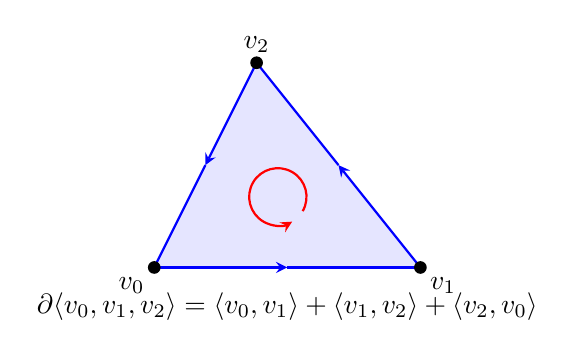
\begin{tikzpicture}[scale=1.3]
        \fill[blue!10] (0,0) -- (2.6,0) -- (1.0,2.0) -- cycle;
        \draw[thick, ->, >=stealth, blue] (0,0) -- (1.3,0);
        \draw[thick, blue] (1.3,0) -- (2.6,0);
        \draw[thick, ->, >=stealth, blue] (2.6,0) -- (1.8,1.0);
        \draw[thick, blue] (1.8,1.0) -- (1.0,2.0);
        \draw[thick, ->, >=stealth, blue] (1.0,2.0) -- (0.5,1.0);
        \draw[thick, blue] (0.5,1.0) -- (0,0);
        \draw[->, >=stealth, thick, red] (1.45,0.55) arc (-30:300:0.28);
        \filldraw (0,0) circle (1.6pt) node[below left] {$v_0$};
        \filldraw (2.6,0) circle (1.6pt) node[below right] {$v_1$};
        \filldraw (1.0,2.0) circle (1.6pt) node[above] {$v_2$};
        \node[below] at (1.3,-0.15) {$\partial \langle v_0,v_1,v_2\rangle = \langle v_0,v_1\rangle + \langle v_1,v_2\rangle + \langle v_2,v_0\rangle$};
    \end{tikzpicture}
    \caption{Il bordo di un triangolo orientato \`e il cammino chiuso formato dai suoi tre lati, percorsi nel verso indotto dall'orientazione.}
\end{figure}


% ======== NUOVO (pp. 157-158) ========
Per costruzione, $\partial_p: C_p(K, \mathbb{Z}) \to C_{p-1}(K, \mathbb{Z})$ \`e un \textbf{omomorfismo di gruppi} e $\partial_p: C_p(K, \mathbb{R}) \to C_{p-1}(K, \mathbb{R})$ \`e un'\textbf{applicazione lineare}.

\begin{observacion}[Buona definizione]
Il bordo $\partial_p \langle v_0, \dots, v_p \rangle$ \`e stato scritto scegliendo un ordinamento dei vertici; bisogna controllare che cambiando orientazione si ottenga il segno opposto, in modo da avere $\partial_p(-\langle s \rangle) = -\partial_p \langle s \rangle$. Basta verificarlo per la trasposizione di due vertici \emph{adiacenti}, $v_j \leftrightarrow v_{j+1}$ (ogni permutazione \`e prodotto di tali trasposizioni): i termini del bordo che omettono un vertice diverso da $v_j, v_{j+1}$ contengono la coppia scambiata e quindi cambiano segno; i due termini che omettono $v_j$ o $v_{j+1}$ sono
\[
(-1)^j \langle \dots, v_{j+1}, \dots \rangle + (-1)^{j+1} \langle \dots, v_j, \dots \rangle \quad \longmapsto \quad (-1)^j \langle \dots, v_j, \dots \rangle + (-1)^{j+1} \langle \dots, v_{j+1}, \dots \rangle ,
\]
che \`e l'opposto del primo. Dunque il bordo cambia segno.
\end{observacion}

\begin{ejemplo}
\begin{enumerate}
    \item $p = 0$: $C_{-1}(K) = 0$, quindi $\partial_0: C_0(K) \to C_{-1}(K) = 0$ \`e l'applicazione nulla ($c \mapsto 0$).
    \item $p = 1$, $\langle s \rangle = \langle v_0, v_1 \rangle$: $\partial_1 \langle v_0, v_1 \rangle = (-1)^0 \langle v_1 \rangle + (-1)^1 \langle v_0 \rangle = \langle v_1 \rangle - \langle v_0 \rangle$; e $\partial_1 \langle v_1, v_0 \rangle = \langle v_0 \rangle - \langle v_1 \rangle$.
    \item $p = 2$, $\langle s \rangle = \langle v_0, v_1, v_2 \rangle$:
    \[
    \partial_2 \langle s \rangle = (-1)^0 \langle v_1, v_2 \rangle + (-1)^1 \langle v_0, v_2 \rangle + (-1)^2 \langle v_0, v_1 \rangle = \langle v_0, v_1 \rangle + \langle v_1, v_2 \rangle + \langle v_2, v_0 \rangle,
    \]
    perch\'e $-\langle v_0, v_2 \rangle = \langle v_2, v_0 \rangle$.
\end{enumerate}
\end{ejemplo}

\begin{lema}
$\partial^2 = 0$, cio\`e $\partial_{p-1} \circ \partial_p = 0$ per ogni $p$.
\end{lema}

\begin{intuizione}
``Il bordo di un bordo \`e vuoto'': il bordo di un triangolo \`e un cammino chiuso, e un cammino chiuso non ha bordo (ogni vertice compare una volta come punto finale e una come punto iniziale, con segni opposti). \`E l'identit\`a che permette di definire l'omologia.
\end{intuizione}

\begin{proof}
Poich\'e $\partial_p$ \`e un omomorfismo di gruppi, basta mostrare che $(\partial_{p-1} \circ \partial_p) \langle s \rangle = 0$ per ogni $p$-simplesso orientato $\langle s \rangle = \langle v_0, \dots, v_p \rangle$. Si ha
\[
\partial_{p-1} \partial_p \langle s \rangle = \sum_{i=0}^p (-1)^i\, \partial_{p-1} \langle v_0, \dots, \widehat{v_i}, \dots, v_p \rangle .
\]
Nel simplesso $\langle v_0, \dots, \widehat{v_i}, \dots, v_p \rangle$ i vertici con indice $j < i$ hanno posizione $j$, quelli con $j > i$ hanno posizione $j - 1$. Quindi
\[
\partial_{p-1} \langle v_0, \dots, \widehat{v_i}, \dots, v_p \rangle = \sum_{j < i} (-1)^j \langle \dots, \widehat{v_j}, \dots, \widehat{v_i}, \dots \rangle + \sum_{j > i} (-1)^{j-1} \langle \dots, \widehat{v_i}, \dots, \widehat{v_j}, \dots \rangle .
\]
Perci\`o
\[
\partial_{p-1} \partial_p \langle s \rangle = \sum_{j < i} (-1)^{i+j} \langle \dots, \widehat{v_j}, \dots, \widehat{v_i}, \dots \rangle + \sum_{i < j} (-1)^{i+j-1} \langle \dots, \widehat{v_i}, \dots, \widehat{v_j}, \dots \rangle .
\]
Nella seconda somma si scambiano i nomi degli indici ($i \leftrightarrow j$): diventa $\sum_{j < i} (-1)^{i+j-1} \langle \dots, \widehat{v_j}, \dots, \widehat{v_i}, \dots \rangle$. Allora le due somme hanno gli stessi addendi con segni opposti e
\[
\partial_{p-1} \partial_p \langle s \rangle = \sum_{j < i} \big( (-1)^{i+j} + (-1)^{i+j-1} \big) \langle \dots, \widehat{v_j}, \dots, \widehat{v_i}, \dots \rangle = 0 . \qquad \square
\]
\end{proof}

\begin{ejemplo}
Per il triangolo: $\partial_1 \partial_2 \langle v_0, v_1, v_2 \rangle = \partial_1 \big( \langle v_0, v_1 \rangle + \langle v_1, v_2 \rangle + \langle v_2, v_0 \rangle \big) = (\langle v_1 \rangle - \langle v_0 \rangle) + (\langle v_2 \rangle - \langle v_1 \rangle) + (\langle v_0 \rangle - \langle v_2 \rangle) = 0$.
\end{ejemplo}


% ======== NUOVO (pp. 159-160) ========
\section{I gruppi di omologia simpliciale}

\begin{definicion}[Cicli e bordi]
Una $p$-catena $c \in C_p(K)$ si dice
\begin{itemize}
    \item \textbf{$p$-ciclo} se $\partial_p c = 0$;
    \item \textbf{$p$-bordo} se esiste $c' \in C_{p+1}(K)$ tale che $c = \partial_{p+1} c'$.
\end{itemize}
\end{definicion}

\begin{observacion}
Per il lemma $\partial^2 = 0$, ogni $p$-bordo \`e anche un $p$-ciclo: se $c = \partial_{p+1} c'$ allora $\partial_p c = \partial_p \partial_{p+1} c' = 0$.
\end{observacion}

\begin{definicion}[Gruppi dei cicli e dei bordi]
Il sottogruppo
\[
Z_p(K) = \{ c \in C_p(K) \mid c \text{ \`e un $p$-ciclo} \} = \operatorname{Ker} \partial_p
\]
si chiama \textbf{gruppo dei $p$-cicli} di $K$. Il sottogruppo
\[
B_p(K) = \{ c \in C_p(K) \mid c \text{ \`e un $p$-bordo} \} = \operatorname{Im} \partial_{p+1}
\]
si chiama \textbf{gruppo dei $p$-bordi}.
\end{definicion}

\begin{observacion}
Per il lemma, $B_p(K) \subseteq Z_p(K)$; poich\'e i gruppi sono abeliani, $B_p(K) \trianglelefteq Z_p(K)$.
\end{observacion}

\begin{definicion}[Omologia simpliciale]
Sia $K$ un complesso simpliciale e $0 \leqslant p \leqslant m = \dim K$. Si chiama \textbf{$p$-esimo gruppo di omologia simpliciale} di $K$ il gruppo quoziente
\[
H_p(K) = \frac{Z_p(K)}{B_p(K)} .
\]
\end{definicion}

\begin{intuizione}
I $p$-cicli sono le ``$p$-superfici senza bordo'' (ad esempio un cammino chiuso per $p=1$); i $p$-bordi sono quelli che si ottengono come bordo di qualcosa di dimensione $p+1$ \emph{presente} in $K$ (cicli che si possono ``riempire''). $H_p(K)$ misura i cicli che \emph{non} si riempiono, cio\`e i ``buchi $p$-dimensionali'' di $K$: componenti connesse per $p=0$, buchi circolari per $p=1$, cavit\`a per $p=2$.
\end{intuizione}

\begin{observacion}
\begin{enumerate}
    \item[0)] $H_p(K) = 0 \iff Z_p(K) = B_p(K) \iff$ ogni $p$-ciclo \`e un $p$-bordo.
    \item[1)] $H_p(K)$ \`e definito per ogni $p \in \mathbb{Z}$, con $H_p(K) = 0$ per $p < 0$ e per $p > \dim K$ (perch\'e $C_p(K) = 0$).
    \item[2)] $C_p(K, \mathbb{Z})$ \`e un gruppo abeliano libero di tipo finito (di rango $l_p$). Ne segue che $Z_p(K, \mathbb{Z}) \leqslant C_p(K, \mathbb{Z})$ \`e un gruppo abeliano libero di tipo finito (un sottogruppo di un gruppo abeliano libero di tipo finito \`e libero di tipo finito). Allora $H_p(K, \mathbb{Z}) = Z_p(K, \mathbb{Z}) / B_p(K, \mathbb{Z})$ \`e abeliano, di tipo finito, ma \textbf{non necessariamente libero}! Per il teorema fondamentale sui gruppi abeliani di tipo finito,
    \[
    H_p(K, \mathbb{Z}) = \beta_p(K, \mathbb{Z}) \oplus \Gamma_p(K, \mathbb{Z}),
    \]
    dove $\beta_p(K, \mathbb{Z})$ \`e libero e $\Gamma_p(K, \mathbb{Z})$ \`e il sottogruppo di torsione.
\end{enumerate}
\end{observacion}

\begin{definicion}[Gruppo di Betti, torsione e numeri di Betti]
\begin{itemize}
    \item $\beta_p(K, \mathbb{Z})$ si chiama \textbf{$p$-esimo gruppo di Betti} di $K$ (da non confondere con $B_p(K)$, il gruppo dei bordi);
    \item $\Gamma_p(K, \mathbb{Z})$ si chiama \textbf{$p$-esimo gruppo di torsione} di $K$;
    \item $\operatorname{rango}\big(H_p(K, \mathbb{Z})\big) = \operatorname{rango}\big(\beta_p(K, \mathbb{Z})\big) = b_p(K)$ si chiama \textbf{$p$-esimo numero di Betti} di $K$.
\end{itemize}
\end{definicion}

\begin{intuizione}
Il numero di Betti $b_p(K)$ conta \emph{quanti} buchi $p$-dimensionali indipendenti ha $K$; la torsione $\Gamma_p$ rileva fenomeni pi\`u sottili (come il ``mezzo giro'' del piano proiettivo, dove $H_1(\mathbb{R}P^2) = \mathbb{Z}_2$).
\end{intuizione}


% ======== NUOVO (pp. 161-166, 29/10/2026) ========
\begin{observacion}[Omologia a coefficienti reali]
$C_p(K, \mathbb{R})$ \`e uno spazio vettoriale reale di dimensione finita $l_p$; quindi $Z_p(K, \mathbb{R}) \subseteq C_p(K, \mathbb{R})$ \`e un sottospazio, e $H_p(K, \mathbb{R}) = Z_p(K, \mathbb{R}) / B_p(K, \mathbb{R})$ \`e uno spazio vettoriale reale di dimensione finita. $H_p(K, \mathbb{Z})$ \`e ``pi\`u ricco'' di $H_p(K, \mathbb{R})$ (contiene anche la torsione, che i coefficienti reali non vedono). Si dimostra che
\[
\dim H_p(K, \mathbb{R}) = \operatorname{rango} H_p(K, \mathbb{Z}) = b_p(K).
\]
\end{observacion}

\section{Componenti connesse di $|K|$}

Sia $K$ un complesso simpliciale e $v, w \in K^0$ vertici. Poniamo
\[
v \sim w \iff \exists\, n \in \mathbb{N}_0,\ \exists\, v_1, \dots, v_n \in K^0 : \ \langle v, v_1 \rangle + \langle v_1, v_2 \rangle + \dots + \langle v_{n-1}, v_n \rangle + \langle v_n, w \rangle \in C_1(K),
\]
cio\`e: $v$ e $w$ si possono collegare con una \textbf{spezzata} di spigoli di $K$ ($v \to v_1 \to \dots \to v_n \to w$, ogni tratto \`e un $1$-simplesso di $K$; per $n = 0$ \`e un solo spigolo, e si conviene $v \sim v$).

\begin{figure}[H]
    \centering
    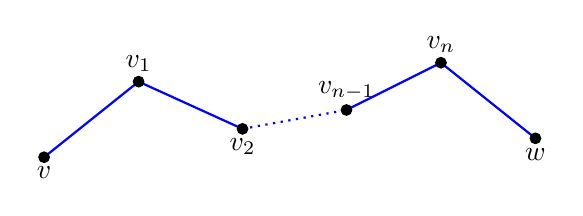
\begin{tikzpicture}[scale=1.2]
        \draw[thick, blue] (0,0) -- (1,0.8) -- (2.1,0.3);
        \draw[thick, blue, dotted] (2.1,0.3) -- (3.2,0.5);
        \draw[thick, blue] (3.2,0.5) -- (4.2,1.0) -- (5.2,0.2);
        \foreach \p/\n/\d in {(0,0)/v/below, (1,0.8)/v_1/above, (2.1,0.3)/v_2/below, (3.2,0.5)/v_{n-1}/above, (4.2,1.0)/v_n/above, (5.2,0.2)/w/below}
            \filldraw \p circle (1.6pt) node[\d] {$\n$};
    \end{tikzpicture}
    \caption{$v \sim w$ se si pu\`o andare da $v$ a $w$ seguendo spigoli del complesso.}
\end{figure}

$\sim$ \`e una \textbf{relazione di equivalenza} su $K^0$:
\begin{itemize}
    \item \emph{riflessiva}: $\langle v, v \rangle = 0 \in C_1(K)$ (cammino di lunghezza zero), quindi $v \sim v$;
    \item \emph{simmetrica}: se $v \sim w$ si percorre la spezzata al contrario: $\langle w, v_n \rangle + \dots + \langle v_1, v \rangle \in C_1(K)$ perch\'e $\langle a, b \rangle = -\langle b, a \rangle$;
    \item \emph{transitiva}: se $v \sim w$ e $w \sim w'$ si concatenano le due spezzate.
\end{itemize}

\begin{observacion}
Se $K = \{ (v_0), (v_1) \}$ (due punti isolati, un complesso simpliciale), allora $v_0 \not\sim v_1$: i due vertici non sono connessi tra loro.
\end{observacion}

\begin{definicion}
Sia $K$ un complesso simpliciale e $v \in K^0$. Poniamo
\[
K_v = \bigcup_{\substack{w \in K^0 \\ w \sim v}} \operatorname{st}(w) = \bigcup_{\substack{(s) \in K \\ (s) \text{ ha un vertice} \sim v}} (s).
\]
\end{definicion}

\begin{prop}[Propriet\`a di $K_v$]
\begin{enumerate}
    \item[1)] Se $(s) \in K$ e $v, w$ sono vertici di $(s)$, allora $v \sim w$.
    \item[2)] $|K| = \bigcup_{v \in K^0} K_v$.
    \item[3)] Se $(s) \subseteq K_v$, allora $[s] \subseteq K_v$.
    \item[4)] $K_v$ \`e un aperto di $|K|$.
    \item[5)] $K_v \neq \varnothing$.
    \item[6)] $K_v = K_{v'} \iff v \sim v'$.
    \item[7)] $K_v$ \`e connesso per archi.
    \item[8)] $K_v \cap K_{v'} \neq \varnothing \iff K_v = K_{v'}$.
    \item[9)] $K_v$ \`e chiuso in $|K|$.
\end{enumerate}
\end{prop}

\begin{proof}
\textbf{1)} Se $(s) \in K$, allora $[s] \subseteq |K|$ e i suoi vertici $v = v_i$, $w = v_j$ sono collegati dal segmento $\overline{v_i v_j}$, che \`e una faccia (spigolo) di $[s]$, quindi un $1$-simplesso di $K$ (condizione 1 di complesso): $v \sim w$.

\textbf{2)} ``$\supseteq$'' \`e banale; ``$\subseteq$'': $|K| = \bigcup_{v \in K^0} \operatorname{st}(v) \subseteq \bigcup_{v} K_v$.

\textbf{3)} Se $(s) \subseteq K_v = \bigcup_{w \sim v} \operatorname{st}(w)$, allora $(s)$ ha un vertice $w \sim v$. Per 1), ogni vertice di $(s)$ \`e equivalente a $w$, e quindi a $v$. Dunque ogni faccia di $[s]$ ha un vertice equivalente a $v$ e $[s] = \bigcup_{(s') \text{ faccia di } (s)} (s') \subseteq K_v$.

\textbf{4)} $K_v = \bigcup_{w \sim v} \operatorname{st}(w)$ \`e unione di aperti (le stelle sono aperte).

\textbf{5)} $v \in K_v$.

\textbf{6)} ($\Rightarrow$) $K_v = K_{v'}$: allora $v \in K_{v'} = \bigcup_{w \sim v'} \operatorname{st}(w)$, quindi esiste $(s) \in K$ con $v \in (s)$ e $(s)$ ha un vertice $\sim v'$. Ma $v \in K^0$ implica $(s) = (v) = \{v\}$, quindi $v \sim v'$. ($\Leftarrow$) Se $v \sim v'$: $x \in K_v \iff \exists w \in K^0: x \in \operatorname{st}(w),\ w \sim v \iff \exists w: x \in \operatorname{st}(w),\ w \sim v' \iff x \in K_{v'}$.

\textbf{7)} Basta mostrare che per ogni $x \in K_v$ esiste un arco che congiunge $x$ a $v$. Sia $x \in K_v$: esiste $(s) \in K$ con $x \in (s)$ e $(s)$ ha un vertice $w \sim v$. Per 3), $[s] \subseteq K_v$ e $[s]$ \`e convesso, quindi $\overline{x, w} \subseteq [s] \subseteq K_v$. Inoltre $w \sim v$ d\`a una spezzata $v \to v_1 \to \dots \to v_n \to w$ di spigoli, con $v_i \sim v$ per ogni $i$; ciascuno spigolo ha un vertice $\sim v$, quindi sta in $K_v$ (per 3)). Allora $\gamma = \overline{x, w} \cup \overline{w, v_n} \cup \dots \cup \overline{v_1, v}$ \`e una spezzata contenuta in $K_v$ che congiunge $x$ a $v$.

\textbf{8)} ($\Leftarrow$) \`E banale per 5). ($\Rightarrow$) Sia $x \in K_v \cap K_{v'}$ e $(s)$ l'unico simplesso aperto con $x \in (s)$. Da $x \in K_v$, $(s)$ ha un vertice $w \sim v$; da $x \in K_{v'}$, ha un vertice $w' \sim v'$. Per 1), $w \sim w'$, quindi $v \sim w \sim w' \sim v'$ e per 6) $K_v = K_{v'}$.

\textbf{9)} Per 2) e 8), $K_v = |K| \setminus \bigcup_{v' \not\sim v} K_{v'}$, complementare di un'unione di aperti (4), dunque chiuso\hfill$\square$
\end{proof}

\begin{prop}
$\{ K_v \}_{v \in K^0}$ \`e l'insieme delle \textbf{componenti connesse (per archi)} di $|K|$.
\end{prop}
\begin{proof}
Per ogni $v \in K^0$, $K_v$ \`e aperto, chiuso, non vuoto e connesso per archi; inoltre due insiemi $K_v$ distinti sono disgiunti (propriet\`a 8) e ricoprono $|K|$ (propriet\`a 2). Dunque sono esattamente le componenti connesse per archi\hfill$\square$
\end{proof}

\begin{coro}
$|K|$ \`e connesso $\iff$ $v \sim v'$ per ogni $v, v' \in K^0$.
\end{coro}
\begin{proof}
Per la proposizione le componenti connesse di $|K|$ sono i $K_v$. Dunque $|K|$ \`e connesso $\iff |K| = K_v = \bigcup_{w \sim v} \operatorname{st}(w)$ per un (ogni) $v$ $\iff$ ogni $w \in K^0$ \`e equivalente a $v$\hfill$\square$
\end{proof}

\begin{intuizione}
$|K|$ \`e connesso se e solo se il ``grafo'' formato dai vertici e dagli spigoli di $K$ \`e connesso. Le componenti connesse sono gli ``isolotti'' separati.
\end{intuizione}

Poniamo $K'_v = \{ (s) \in K \mid (s) \subseteq K_v \} \subseteq K$.

\begin{prop}
$K'_v$ \`e un complesso simpliciale (con sostegno $|K'_v| = K_v$).
\end{prop}
\begin{proof}
La condizione 2) di complesso (due simplessi aperti distinti sono disgiunti) \`e banale perch\'e $K'_v \subseteq K$. Per la condizione 1): se $(s) \in K'_v$ e $(s')$ \`e una faccia aperta di $(s)$, allora $(s') \subseteq [s] \subseteq K_v$ (per 3)), cio\`e $(s') \in K'_v$\hfill$\square$
\end{proof}


% ======== NUOVO (pp. 167-174) ========
\begin{teo}
Sia $K$ un complesso simpliciale e siano $K_1, \dots, K_n$ i complessi $K'_{v}$ associati alle componenti connesse di $|K|$ (cio\`e $|K_i|$ sono le componenti connesse di $|K|$). Allora, per ogni $p$,
\[
H_p(K) \cong \bigoplus_{i=1}^n H_p(K_i) .
\]
\end{teo}
\begin{proof}
Per ogni $p$ vale $C_p(K) = C_p(K_1) \oplus \dots \oplus C_p(K_n)$: ogni $p$-simplesso di $K$ \`e contenuto in uno e uno solo dei sottoinsiemi $|K_i|$, quindi ogni $p$-catena di $K$ si decompone in modo unico come somma di $p$-catene dei vari $K_i$. Il bordo di un simplesso di $K_i$ \`e una catena di $K_i$ (le facce di un simplesso stanno nella stessa componente), quindi, essendo $\partial_p$ un omomorfismo,
\[
B_p(K) = \partial_{p+1}\big(C_{p+1}(K)\big) = \partial_{p+1}\big(C_{p+1}(K_1) \oplus \dots \oplus C_{p+1}(K_n)\big) = B_p(K_1) \oplus \dots \oplus B_p(K_n) .
\]
Inoltre, se $c \in Z_p(K)$, $c = c_1 + \dots + c_n$ con $c_i \in C_p(K_i)$, e $0 = \partial_p c = \partial_p c_1 + \dots + \partial_p c_n$, con $\partial_p c_i \in C_{p-1}(K_i)$ in addendi diversi di una somma diretta; ne segue $\partial_p c_i = 0$, cio\`e $c_i \in Z_p(K_i)$ per ogni $i$. Dunque $Z_p(K) = Z_p(K_1) \oplus \dots \oplus Z_p(K_n)$ e
\[
H_p(K) = \frac{Z_p(K)}{B_p(K)} = \frac{Z_p(K_1) \oplus \dots \oplus Z_p(K_n)}{B_p(K_1) \oplus \dots \oplus B_p(K_n)} \cong \frac{Z_p(K_1)}{B_p(K_1)} \oplus \dots \oplus \frac{Z_p(K_n)}{B_p(K_n)} = H_p(K_1) \oplus \dots \oplus H_p(K_n). \qquad \square
\]
\end{proof}

\section{Omologia $0$-dimensionale}

\begin{teo}
Sia $K$ un complesso simpliciale e sia $n$ il numero delle componenti connesse di $|K|$. Allora
\[
H_0(K, \mathbb{Z}) \cong \mathbb{Z}^n \qquad \big( \text{e } H_0(K, \mathbb{R}) \cong \mathbb{R}^n \big).
\]
\end{teo}

\begin{intuizione}
$H_0$ \emph{conta le componenti connesse}: $b_0(K) = n$. \`E il primo caso concreto in cui un gruppo di omologia misura una caratteristica geometrica elementare.
\end{intuizione}

\begin{proof}
Per il teorema precedente basta supporre $|K|$ connesso e provare che $H_0(K, \mathbb{R}) \cong \mathbb{R}$ (e $H_0(K, \mathbb{Z}) \cong \mathbb{Z}$). Poich\'e $\partial_0 = 0$, $Z_0 = C_0$ e $H_0(K, \mathbb{R}) = C_0(K, \mathbb{R}) / B_0(K, \mathbb{R})$. Sia $K^0 = \{ v_1, \dots, v_{l_0} \}$ e consideriamo
\[
\varphi: C_0(K, \mathbb{R}) \to \mathbb{R}, \qquad c = \sum_{i=1}^{l_0} \alpha_i \langle v_i \rangle \longmapsto \sum_{i=1}^{l_0} \alpha_i
\]
(la somma dei coefficienti). \`E un omomorfismo, ed \`e suriettivo perch\'e $\varphi(k \langle v_i \rangle) = k$ per ogni $k \in \mathbb{R}$. Per il teorema di isomorfismo $C_0(K, \mathbb{R}) / \operatorname{Ker} \varphi \cong \mathbb{R}$. Mostriamo che $\operatorname{Ker} \varphi = B_0(K, \mathbb{R})$.

$(\subseteq)$ Sia $c = \sum \alpha_i \langle v_i \rangle \in \operatorname{Ker} \varphi$, cio\`e $\sum \alpha_i = 0$. Fissato $v_0 \in K^0$:
\[
c = \sum_i \alpha_i \langle v_i \rangle - \Big( \sum_i \alpha_i \Big) \langle v_0 \rangle = \sum_{i} \alpha_i \big( \langle v_i \rangle - \langle v_0 \rangle \big).
\]
Poich\'e $|K|$ \`e connesso, $v_i \sim v_0$ per ogni $i$: esiste una spezzata di spigoli da $v_0$ a $v_i$, cio\`e una $1$-catena $c_i' \in C_1(K, \mathbb{R})$ con $\partial_1 c'_i = \langle v_i \rangle - \langle v_0 \rangle$ (la somma lungo il cammino ``telescopizza''). Allora $c = \sum_i \alpha_i \partial_1 c'_i = \partial_1 \big( \sum_i \alpha_i c'_i \big) \in B_0(K, \mathbb{R})$.

$(\supseteq)$ Se $c \in B_0(K, \mathbb{R})$, $c = \partial_1 c_1$ con $c_1 = \sum_j a_j \langle v_j, w_j \rangle$, quindi $c = \sum_j a_j (\langle w_j \rangle - \langle v_j \rangle)$ e $\varphi(c) = \sum a_j - \sum a_j = 0$.

Dunque $H_0(K, \mathbb{R}) = C_0(K, \mathbb{R}) / B_0(K, \mathbb{R}) = C_0 / \operatorname{Ker} \varphi \cong \mathbb{R}$\hfill$\square$
\end{proof}

\begin{ejemplo}
Se $K$ \`e un triangolo pieno (connesso), $H_0(K) \cong \mathbb{Z}$; se $K = \{ (v_0), (v_1) \}$ (due punti) allora $H_0(K) \cong \mathbb{Z}^2$.
\end{ejemplo}

\section{Invarianza topologica dei gruppi di omologia simpliciale}

\begin{teo}
Siano $K, L$ complessi simpliciali. Se $|K| \overset{\text{top}}{\cong} |L|$ (omeomorfi), allora $H_p(K) \overset{\text{alg}}{\cong} H_p(L)$ per ogni $p$.
\end{teo}

\begin{observacion}
\`E il risultato che giustifica l'uso dell'omologia come invariante topologico: \emph{non dipende dalla triangolazione scelta}, ma solo dallo spazio $|K|$. Gli appunti ne danno lo \textbf{schema} della dimostrazione; per i dettagli si veda S.~R.~Munkres, \emph{Elements of Algebraic Topology}.
\end{observacion}

\textbf{Schema della dimostrazione.}

\medskip
\textbf{I passo: applicazioni simpliciali e omologia.} Siano $K, L$ complessi simpliciali. Un'applicazione $f: |K| \to |L|$ si dice \textbf{applicazione simpliciale} se manda $p$-simplessi di $K$ in $q$-simplessi di $L$, con $q \leqslant p$. In particolare, per ogni $v \in K^0$ si ha $f(v) \in L^0$ e $f$ si ottiene estendendo ``linearmente'' la sua azione sui vertici:
\[
f: |K| \to |L|, \qquad x = \sum_{v \in K^0} t_v(x)\, v \ \longmapsto\ \sum_{v \in K^0} t_v(x)\, f(v) .
\]
Se $f$ \`e simpliciale, essa induce un omomorfismo di gruppi
\[
f_{\#p}: C_p(K) \to C_p(L), \qquad \langle v_0, \dots, v_p \rangle \longmapsto \begin{cases} 0 & \text{se } f(v_0), \dots, f(v_p) \text{ non sono c-indip.,} \\ \langle f(v_0), \dots, f(v_p) \rangle & \text{se sono c-indipendenti,} \end{cases}
\]
esteso per linearit\`a a tutte le $p$-catene. Si dimostra che $f_\#$ commuta con il bordo: $\partial_p \circ f_{\#p} = f_{\#, p-1} \circ \partial_p$ (diagramma commutativo). Ne segue facilmente che $f_{\#p}$ manda $p$-cicli in $p$-cicli e $p$-bordi in $p$-bordi, quindi induce un omomorfismo di gruppi
\[
f_{*p}: H_p(K) \to H_p(L), \qquad [c] \longmapsto [f_{\#p}\, c] .
\]

\textbf{II passo: applicazioni contigue.} Due applicazioni simpliciali $f, g: |K| \to |L|$ si dicono \textbf{contigue} se per ogni $p$-simplesso $\langle v_0, \dots, v_p \rangle$ di $K$ i vertici $f(v_0), \dots, f(v_p), g(v_0), \dots, g(v_p)$ generano un simplesso di $L$ (di dimensione al pi\`u $2p+1$). Si dimostra che se $f, g$ sono continue e contigue allora $f_{*p} = g_{*p}$ per ogni $p$ (con un argomento di omotopia di catene).

\textbf{III passo: approssimazione simpliciale.} Sia $f: |K| \to |L|$ continua. Si dimostra che esiste una suddivisione baricentrica $K' = K^{(n)}$ di $K$ tale che per ogni $v \in (K')^0$ esiste $u \in L^0$ con $f(\operatorname{st}(v)) \subseteq \operatorname{st}(u)$. (Si usa il numero di Lebesgue per il ricoprimento $\{ f^{-1}(\operatorname{st}(u)) \}_{u \in L^0}$ di $|K|$ e il fatto che la maglia di $K^{(n)}$ tende a $0$.) Si pone allora
\[
h: (K')^0 \to L^0, \quad v \mapsto u \text{ tale che } f(\operatorname{st}(v)) \subseteq \operatorname{st}(u),
\]
e si estende $h$ a tutto $|K'| = |K|$ ponendo $h(x) = \sum_{v \in (K')^0} t_v(x)\, h(v)$. L'applicazione $h$ si chiama \textbf{approssimazione simpliciale} di $f$. Si dimostra che se $h, g$ sono entrambe approssimazioni simpliciali di $f$, allora $h$ e $g$ sono contigue e quindi $h_{*p} = g_{*p}$ per ogni $p$. Inoltre:
\begin{enumerate}
    \item[a)] l'identit\`a (continua) $\mathrm{Id}: |K'| \to |K|$ ha un'approssimazione simpliciale $\Phi$ tale che $\Phi_{*p}: H_p(K') \to H_p(K)$ \`e un \textbf{isomorfismo} per ogni $p$ (l'omologia non cambia per suddivisione baricentrica).
\end{enumerate}
Per definizione si pone allora
\[
f_{*p} = h_{*p} \circ \Phi_{*p}^{-1}: \ H_p(K) \xrightarrow{\ \Phi_{*p}^{-1}\ } H_p(K') \xrightarrow{\ h_{*p}\ } H_p(L).
\]
\begin{enumerate}
    \item[b)] L'identit\`a $\mathrm{Id}: |K| \to |K|$ induce l'identit\`a $\mathrm{Id}_{*p}: H_p(K) \to H_p(K)$ per ogni $p$, e date $f: |K| \to |L|$, $g: |L| \to |M|$ continue, $(g \circ f)_{*p} = g_{*p} \circ f_{*p}$ (funtorialit\`a).
\end{enumerate}

\begin{figure}[H]
    \centering
    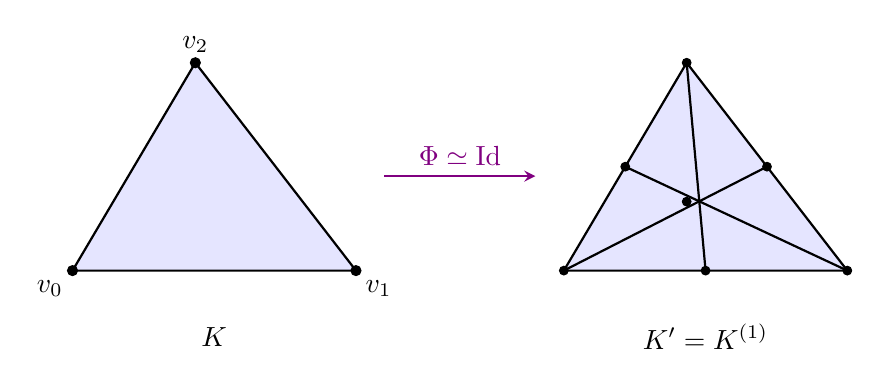
\begin{tikzpicture}[scale=1.2]
        \begin{scope}
            \fill[blue!10] (0,0) -- (3,0) -- (1.3,2.2) -- cycle;
            \draw[thick] (0,0) -- (3,0) -- (1.3,2.2) -- cycle;
            \filldraw (0,0) circle (1.5pt) node[below left] {$v_0$};
            \filldraw (3,0) circle (1.5pt) node[below right] {$v_1$};
            \filldraw (1.3,2.2) circle (1.5pt) node[above] {$v_2$};
            \node at (1.5,-0.7) {$K$};
        \end{scope}
        \begin{scope}[shift={(5.2,0)}]
            \fill[blue!10] (0,0) -- (3,0) -- (1.3,2.2) -- cycle;
            \draw[thick] (0,0) -- (3,0) -- (1.3,2.2) -- cycle;
            \draw[thick] (0,0) -- (2.15,1.1); \draw[thick] (3,0) -- (0.65,1.1); \draw[thick] (1.3,2.2) -- (1.5,0);
            \foreach \p in {(0,0),(3,0),(1.3,2.2),(1.5,0),(0.65,1.1),(2.15,1.1),(1.3,0.73)} \filldraw \p circle (1.3pt);
            \node at (1.5,-0.7) {$K' = K^{(1)}$};
        \end{scope}
        \draw[->, >=stealth, thick, Purple] (3.3,1.0) -- (4.9,1.0) node[midway, above] {$\Phi \simeq \mathrm{Id}$};
    \end{tikzpicture}
    \caption{Il ciclo $\langle v_0,v_1\rangle + \langle v_1,v_2\rangle + \langle v_2,v_0\rangle = \partial_2 \langle v_0,v_1,v_2\rangle$ si manda in modo naturale nel ciclo analogo di $K'$ (suddiviso): $\Phi_*$ \`e un isomorfismo.}
\end{figure}

\textbf{IV passo: conclusione.} Sia $f: |K| \to |L|$ un omeomorfismo: $f$ e $f^{-1}$ sono continue e $f^{-1} \circ f = \mathrm{Id}_{|K|}$, $f \circ f^{-1} = \mathrm{Id}_{|L|}$. Per la funtorialit\`a e il punto b),
\[
(f^{-1} \circ f)_{*p} = (\mathrm{Id}_{|K|})_{*p}, \qquad (f \circ f^{-1})_{*p} = (\mathrm{Id}_{|L|})_{*p},
\]
cio\`e $f^{-1}_{*p} \circ f_{*p} = \mathrm{Id}_{H_p(K)}$ e $f_{*p} \circ f^{-1}_{*p} = \mathrm{Id}_{H_p(L)}$. Dunque $f_{*p}: H_p(K) \to H_p(L)$ \`e un \textbf{isomorfismo} (con inverso $(f^{-1})_{*p}$)\hfill$\square$

\begin{intuizione}
Il punto chiave \`e che l'omologia \`e definita a partire da una \emph{triangolazione}, ma applicazioni continue qualsiasi tra gli spazi $|K|$ e $|L|$ possono essere ``approssimate'' da applicazioni simpliciali (dopo aver suddiviso abbastanza), e le approssimazioni diverse inducono la stessa applicazione in omologia.
\end{intuizione}


% ======== NUOVO (pp. 175-176, 3/11) ========
\section{Spazi triangolabili}

\begin{definicion}[Spazio triangolabile]
Uno spazio topologico $X$ si dice \textbf{triangolabile} se esiste un complesso simpliciale $K$ tale che $X \cong |K|$ (nelle notazioni degli appunti: $X = |K|$, a meno di omeomorfismo). Un tale $K$ si chiama una \emph{triangolazione} di $X$.
\end{definicion}

\begin{observacion}
\begin{enumerate}
    \item Se $X$ \`e triangolabile, ha senso definire $H_p(X) = H_p(K)$ per ogni $p$, dove $X = |K|$: per il teorema di invarianza topologica il risultato non dipende dalla triangolazione scelta.
    \item Se $X$ \`e triangolabile, allora $X$ \`e \textbf{compatto} e \textbf{di Hausdorff} ($|K|$ \`e unione finita di simplessi chiusi compatti, ed \`e un sottospazio di $\mathbb{R}^n$). Dunque $\mathbb{R}^n$ o un aperto non possono essere triangolabili.
\end{enumerate}
\end{observacion}

\begin{observacion}[Il viceversa del teorema di invarianza \emph{non} vale]
Se $K, L$ sono complessi simpliciali, allora $|K| \cong |L| \Rightarrow H_p(K) \cong H_p(L)$ per ogni $p$, ma \textbf{non} vale il viceversa.
\end{observacion}

\begin{ejemplo}[Controesempio]
Consideriamo due complessi simpliciali $K$ e $L$ con $H_p(K) \cong H_p(L)$ per ogni $p$ ma $|K| \not\cong |L|$:
\begin{itemize}
    \item $K = \{ (v_0), (v_1), (v_0, v_1) \}$ (un segmento);
    \item $L = \{ (v_0), (v_1), (v_2), (v_3), (v_0, v_1), (v_0, v_2), (v_0, v_3) \}$ (una ``Y'': tre segmenti uscenti da $v_0$).
\end{itemize}
Entrambi hanno dimensione $1$, ma $|K| \not\cong |L|$: togliendo il punto $v_0$ da $|L|$ si ottengono tre componenti connesse, mentre togliendo un punto interno a un segmento si ottengono al pi\`u due.

\begin{figure}[H]
    \centering
    \begin{tikzpicture}[scale=1.2]
        \begin{scope}
            \draw[very thick, blue] (0,0) -- (2,0);
            \filldraw (0,0) circle (2pt) node[below] {$v_0$};
            \filldraw (2,0) circle (2pt) node[below] {$v_1$};
            \node at (1,-0.9) {$|K|$};
        \end{scope}
        \begin{scope}[shift={(5,0)}]
            \draw[very thick, red] (0,0) -- (-1.0,-0.8);
            \draw[very thick, red] (0,0) -- (1.0,-0.8);
            \draw[very thick, red] (0,0) -- (0,1.1);
            \filldraw (0,0) circle (2pt) node[right] {$v_0$};
            \filldraw (-1,-0.8) circle (2pt) node[below] {$v_1$};
            \filldraw (1,-0.8) circle (2pt) node[below] {$v_2$};
            \filldraw (0,1.1) circle (2pt) node[above] {$v_3$};
            \node at (0,-1.7) {$|L|$};
        \end{scope}
    \end{tikzpicture}
    \caption{Un segmento e una ``Y'' non sono omeomorfi, ma hanno la stessa omologia (sono entrambi contraibili).}
\end{figure}

Calcoliamo l'omologia.
\begin{itemize}
    \item $p = 0$: $H_0(K, \mathbb{Z}) = H_0(L, \mathbb{Z}) = \mathbb{Z}$, perch\'e $|K|$ e $|L|$ sono connessi.
    \item $p = 1$, $K$: $H_1(K, \mathbb{Z}) = Z_1(K, \mathbb{Z})$ (non ci sono $2$-simplessi, $B_1 = 0$). Se $c \in Z_1(K, \mathbb{Z})$, $c = \alpha \langle v_0, v_1 \rangle$ con $\alpha \in \mathbb{Z}$ e $0 = \partial_1 c = \alpha(\langle v_1 \rangle - \langle v_0 \rangle) = -\alpha \langle v_0 \rangle + \alpha \langle v_1 \rangle$, da cui $\alpha = 0$, $c = 0$. Quindi $H_1(K, \mathbb{Z}) = 0$.
    \item $p = 1$, $L$: se $c = \alpha \langle v_0, v_1 \rangle + \beta \langle v_0, v_2 \rangle + \gamma \langle v_0, v_3 \rangle \in Z_1(L, \mathbb{Z})$, allora
    \[
    0 = \partial_1 c = \alpha(\langle v_1 \rangle - \langle v_0 \rangle) + \beta(\langle v_2 \rangle - \langle v_0 \rangle) + \gamma(\langle v_3 \rangle - \langle v_0 \rangle) = -(\alpha + \beta + \gamma)\langle v_0 \rangle + \alpha \langle v_1 \rangle + \beta \langle v_2 \rangle + \gamma \langle v_3 \rangle,
    \]
    da cui $\alpha = \beta = \gamma = 0$ e $c = 0$. Quindi $H_1(L, \mathbb{Z}) = Z_1(L, \mathbb{Z}) = 0$.
    \item $p \geqslant 2$: $C_p = 0$, quindi $H_p = 0$ per entrambi.
\end{itemize}
Dunque $H_p(K, \mathbb{Z}) \cong H_p(L, \mathbb{Z})$ per ogni $p$, ma $|K| \not\cong |L|$: l'omologia \`e un invariante topologico \emph{non completo} (distingue meno degli omeomorfismi; \`e invece un invariante di tipo di omotopia).
\end{ejemplo}


% ======== NUOVO (pp. 177-178) ========
\section{Relazione tra $\Pi_1$ e $H_1$}

Sia $K$ un complesso simpliciale con $|K|$ \textbf{connesso} e fissiamo $v_0 \in K^0$.

\medskip
\textbf{Costruzione.} Si dimostra (con l'approssimazione simpliciale, cio\`e deformando il cappio fino a farlo correre lungo gli spigoli di $K$) che per ogni cappio $\sigma \in \Lambda_{v_0}(|K|)$ esiste una $1$-catena $c_\sigma \in C_1(K, \mathbb{Z})$ del tipo
\[
c_\sigma = \langle v_0, v_1 \rangle + \dots + \langle v_{k-1}, v_k \rangle + \langle v_k, v_0 \rangle
\]
(un \emph{cammino chiuso di spigoli}) tale che $\sigma \simeq c_\sigma$ rel $\partial I$ (qui $c_\sigma$ indica anche il cappio poligonale corrispondente).

\begin{figure}[H]
    \centering
    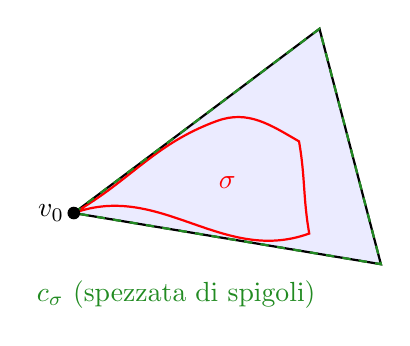
\begin{tikzpicture}[scale=1.3]
        \fill[blue!8] (0,0) -- (3,-0.5) -- (2.4,1.8) -- cycle;
        \draw[thick] (0,0) -- (3,-0.5) -- (2.4,1.8) -- cycle;
        \draw[thick, red] (0,0) to[out=30, in=200] (1.4,0.9) to[out=20, in=150] (2.2,0.7) to[out=-80, in=100] (2.3,-0.2) to[out=200, in=20] (0,0);
        \node[red] at (1.5,0.3) {$\sigma$};
        \draw[thick, ForestGreen, dashed] (0,0) -- (2.4,1.8) -- (3,-0.5) -- cycle;
        \node[ForestGreen] at (1.0,-0.8) {$c_\sigma$ (spezzata di spigoli)};
        \filldraw (0,0) circle (1.6pt) node[left] {$v_0$};
    \end{tikzpicture}
    \caption{Ogni cappio $\sigma$ \`e omotopo (rel $\partial I$) a un cammino chiuso lungo gli spigoli $c_\sigma$.}
\end{figure}

\begin{observacion}
$c_\sigma$ \`e un $1$-ciclo. Infatti
\[
\partial_1 c_\sigma = (\langle v_1 \rangle - \langle v_0 \rangle) + (\langle v_2 \rangle - \langle v_1 \rangle) + \dots + (\langle v_0 \rangle - \langle v_k \rangle) = 0 .
\]
\end{observacion}

Si dimostra inoltre che $\sigma \simeq \tau$ rel $\partial I \implies c_\sigma - c_\tau \in B_1(K, \mathbb{Z})$. Dunque ha senso definire
\[
\varphi: \Pi_1(|K|, v_0) \longrightarrow H_1(K, \mathbb{Z}), \qquad [\sigma]_{\simeq \text{ rel } \partial I} \longmapsto [c_\sigma]_{B_1} .
\]

\begin{prop}[Propriet\`a di $\varphi$]
\begin{enumerate}
    \item $\varphi$ \`e un omomorfismo di gruppi.
    \item $\varphi$ \`e suriettiva.
\end{enumerate}
\end{prop}
\begin{proof}
1) $c_{\sigma * \tau} = c_\sigma + c_\tau$ (il cammino chiuso di spigoli che percorre prima quello di $\sigma$ e poi quello di $\tau$), quindi
\[
\varphi([\sigma][\tau]) = \varphi([\sigma * \tau]) = [c_\sigma + c_\tau]_{B_1} = [c_\sigma]_{B_1} + [c_\tau]_{B_1} = \varphi([\sigma]) + \varphi([\tau]).
\]
2) Sia $[c] \in H_1(K, \mathbb{Z})$. Si dimostra che $[c]_{B_1}$ ha un rappresentante della forma $\langle v_0, v_1 \rangle + \dots + \langle v_k, v_0 \rangle$ (un ciclo di tipo ``cammino chiuso'', usando la connessione di $|K|$ per ricondursi a $v_0$). Allora il cappio poligonale $\sigma = \overline{v_0 v_1} \cup \dots \cup \overline{v_k v_0} \in \Lambda_{v_0}(|K|)$ soddisfa $\varphi([\sigma]) = [\langle v_0, v_1 \rangle + \dots + \langle v_k, v_0 \rangle] = [c]$\hfill$\square$
\end{proof}

Per il teorema di isomorfismo, $\varphi$ induce un isomorfismo di gruppi
\[
\widetilde{\varphi}: \Pi_1(|K|, v_0) / \operatorname{Ker} \varphi \xrightarrow{\ \cong\ } H_1(K, \mathbb{Z}) .
\]
Pi\`u precisamente, si dimostra che $\operatorname{Ker} \varphi$ \`e il derivato $\Pi_1'$ (il sottogruppo dei commutatori), cio\`e
\[
\boxed{ H_1(K, \mathbb{Z}) \cong \Pi_1 / \Pi_1' } ,
\]
\emph{$H_1$ \`e l'abelianizzato di $\Pi_1$} (teorema di Hurewicz in dimensione $1$).

\begin{coro}
Sia $K$ un complesso simpliciale con $|K|$ connesso. Allora $\Pi_1(|K|)$ \`e abeliano se e solo se $\Pi_1(|K|) \cong H_1(K, \mathbb{Z})$.
\end{coro}
\begin{proof}
$\Pi_1$ \`e abeliano $\iff$ $\Pi_1' = \{e\}$ $\iff$ $\Pi_1 / \Pi_1' = \Pi_1$\hfill$\square$
\end{proof}

\begin{ejemplo}[$S^1 \vee S^1$]
Sia $X = S^1 \vee S^1$ (il ``otto''), triangolabile: sia $K$ il complesso con vertici $v_0, v_1, v_2, v_3, v_4$ e spigoli $(v_0, v_1), (v_1, v_2), (v_2, v_0), (v_0, v_3), (v_3, v_4), (v_4, v_0)$ (due triangoli vuoti che condividono il vertice $v_0$), cos\`i $X = |K|$.

\begin{figure}[H]
    \centering
    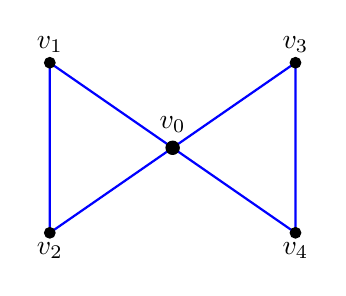
\begin{tikzpicture}[scale=1.2]
        \draw[thick, blue] (0,0) -- (-1.3,0.9) -- (-1.3,-0.9) -- cycle;
        \draw[thick, blue] (0,0) -- (1.3,0.9) -- (1.3,-0.9) -- cycle;
        \filldraw (0,0) circle (2pt) node[above=2pt] {$v_0$};
        \filldraw (-1.3,0.9) circle (1.6pt) node[above] {$v_1$};
        \filldraw (-1.3,-0.9) circle (1.6pt) node[below] {$v_2$};
        \filldraw (1.3,0.9) circle (1.6pt) node[above] {$v_3$};
        \filldraw (1.3,-0.9) circle (1.6pt) node[below] {$v_4$};
    \end{tikzpicture}
    \caption{Una triangolazione di $S^1 \vee S^1$.}
\end{figure}

Allora $\Pi_1(X) = F_2$, che non \`e abeliano, dunque $\Pi_1(X) \not\cong H_1(K, \mathbb{Z})$. Infatti
\[
H_1(X, \mathbb{Z}) = H_1(K, \mathbb{Z}) = F_2 / (F_2)' \cong \mathbb{Z}^2
\]
(l'abelianizzato di $F_2 = \langle a, b \rangle$ \`e $\mathbb{Z}^2$). Verifica diretta: $K$ ha $l_0 = 5$ vertici, $l_1 = 6$ spigoli e nessun $2$-simplesso, quindi $H_1 = Z_1 = \operatorname{Ker}\partial_1$; poich\'e $|K|$ \`e connesso $\operatorname{rango}\operatorname{Im}\partial_1 = 5 - 1 = 4$ e $\operatorname{rango} Z_1 = 6 - 4 = 2$, e $Z_1$ \`e libero (sottogruppo di $\mathbb{Z}^6$): $Z_1 \cong \mathbb{Z}^2$, generato dai due triangoli $\langle v_0, v_1 \rangle + \langle v_1, v_2 \rangle + \langle v_2, v_0 \rangle$ e $\langle v_0, v_3 \rangle + \langle v_3, v_4 \rangle + \langle v_4, v_0 \rangle$.
\end{ejemplo}

\begin{intuizione}
$\Pi_1$ ricorda \emph{in che ordine} si percorrono i cappi (non commutativo: $ab \neq ba$ in $F_2$); $H_1$ ricorda solo \emph{quante volte} si percorre ciascuno (commutativo: $ab = ba$ in $\mathbb{Z}^2$). L'omologia \`e pi\`u debole ma molto pi\`u calcolabile.
\end{intuizione}


% ======== NUOVO (pp. 179-182) ========
\section{Calcolo dei gruppi di omologia: esempi}

\begin{ejercicio*}
Provare per calcolo diretto che $H_1(S^1 \vee S^1, \mathbb{Z}) \cong \mathbb{Z}^2$ (vedi la verifica nell'esempio della sezione precedente).
\end{ejercicio*}

\begin{ejercicio*}
Determinare i gruppi di omologia $H_p(X)$, dove $X$ \`e il seguente spazio triangolabile:
\end{ejercicio*}

\subsection{1) La circonferenza $X = S^1$}

$S^1 = |K|$ con $K = [v_0, v_1, v_2]^1$ (l'$1$-scheletro del triangolo, cio\`e il contorno senza l'interno):
\[
K = \{ (v_0), (v_1), (v_2), (v_0, v_1), (v_1, v_2), (v_0, v_2) \}, \qquad \dim K = 1 .
\]
Quindi dobbiamo calcolare $H_p(S^1) = H_p(K)$ per $p = 0, 1$.
\begin{itemize}
    \item $p = 0$: $H_0(S^1, \mathbb{Z}) = \mathbb{Z}$ (connesso).
    \item $p = 1$: $H_1(S^1, \mathbb{Z}) = \Pi_1(S^1)/\Pi_1(S^1)' = \mathbb{Z}$ (perch\'e $\Pi_1(S^1) = \mathbb{Z}$ \`e abeliano e quindi $\Pi_1' = 0$).
\end{itemize}
\textbf{Calcolo diretto.} Poich\'e $\dim K = 1$, $H_1(S^1, \mathbb{Z}) = H_1(K, \mathbb{Z}) = Z_1(K, \mathbb{Z})$. Sia $c \in C_1(K, \mathbb{Z})$: $c = \alpha \langle v_0, v_1 \rangle + \beta \langle v_1, v_2 \rangle + \gamma \langle v_2, v_0 \rangle$ con $\alpha, \beta, \gamma \in \mathbb{Z}$. Allora
\[
\partial_1 c = \alpha(\langle v_1 \rangle - \langle v_0 \rangle) + \beta(\langle v_2 \rangle - \langle v_1 \rangle) + \gamma(\langle v_0 \rangle - \langle v_2 \rangle) = (\gamma - \alpha)\langle v_0 \rangle + (\alpha - \beta)\langle v_1 \rangle + (\beta - \gamma)\langle v_2 \rangle .
\]
$c \in Z_1 \iff \gamma - \alpha = \alpha - \beta = \beta - \gamma = 0 \iff \alpha = \beta = \gamma$. Dunque
\[
Z_1(K, \mathbb{Z}) = \{ \alpha ( \langle v_0, v_1 \rangle + \langle v_1, v_2 \rangle + \langle v_2, v_0 \rangle ) \mid \alpha \in \mathbb{Z} \} \cong \mathbb{Z} = H_1(S^1, \mathbb{Z}).
\]
(Il generatore \`e il ciclo che percorre la circonferenza una volta.)

\textbf{Riassunto:} $H_0(S^1) = \mathbb{Z}$, $H_1(S^1) = \mathbb{Z}$, $H_p(S^1) = 0$ per $p \geqslant 2$.

\subsection{2) Il disco $X = B^2$}

$B^2 = |K|$ con $K = [v_0, v_1, v_2]$ il triangolo pieno:
\[
K = \{ (v_0), (v_1), (v_2), (v_0, v_1), (v_1, v_2), (v_2, v_0), (v_0, v_1, v_2) \}, \qquad \dim K = 2 .
\]
\begin{itemize}
    \item $p = 0$: $H_0(B^2, \mathbb{Z}) = \mathbb{Z}$ ($B^2$ \`e connesso).
    \item $p = 1$: gli $1$-cicli sono gli stessi di $S^1 = \partial B^2$: $Z_1(K, \mathbb{Z}) = \{ \alpha ( \langle v_0, v_1 \rangle + \langle v_1, v_2 \rangle + \langle v_2, v_0 \rangle ) \} = \{ \alpha\, \partial_2 \langle v_0, v_1, v_2 \rangle \mid \alpha \in \mathbb{Z} \} = B_1(K, \mathbb{Z})$. Ora il ciclo \`e un bordo (il disco ``riempie'' la circonferenza), quindi $H_1(K, \mathbb{Z}) = Z_1/B_1 = 0$. D'altra parte, coerentemente, $\Pi_1(B^2) = 0$ implica $H_1 = \Pi_1/\Pi_1' = 0$.
    \item $p = 2$: $H_2(B^2, \mathbb{Z}) = Z_2(K, \mathbb{Z})$ (non ci sono $3$-simplessi). $c = \alpha \langle v_0, v_1, v_2 \rangle$ e $\partial_2 c = \alpha( \langle v_1, v_2 \rangle - \langle v_0, v_2 \rangle + \langle v_0, v_1 \rangle )$ \`e nullo solo se $\alpha = 0$. Quindi $Z_2 = 0$ e $H_2(B^2, \mathbb{Z}) = 0$.
\end{itemize}
\textbf{Riassunto:} $H_0(B^2) = \mathbb{Z}$, $H_p(B^2) = 0$ per $p \geqslant 1$.

\subsection{3) La sfera $X = S^2$}

$S^2 = |K|$ con $K = [v_0, v_1, v_2, v_3]^2$ (il $2$-scheletro del tetraedro: $4$ vertici, $6$ spigoli, $4$ facce triangolari), $\dim K = 2$.
\begin{itemize}
    \item $p = 0$: $H_0(S^2, \mathbb{Z}) = \mathbb{Z}$ ($S^2$ \`e connessa).
    \item $p = 1$: $\Pi_1(S^2) = 0$, quindi $H_1(S^2, \mathbb{Z}) = \Pi_1/\Pi_1' = 0$ (esercizio: calcolo diretto).
    \item $p = 2 = \dim K$: $H_2(S^2, \mathbb{Z}) = Z_2(K, \mathbb{Z})$. Una $2$-catena \`e $c = \alpha \langle v_0, v_1, v_2 \rangle + \beta \langle v_0, v_1, v_3 \rangle + \gamma \langle v_0, v_2, v_3 \rangle + \delta \langle v_1, v_2, v_3 \rangle$. Poich\'e
    \begin{align*}
    \partial_2 \langle v_0, v_1, v_2 \rangle &= \langle v_1, v_2 \rangle - \langle v_0, v_2 \rangle + \langle v_0, v_1 \rangle, \\
    \partial_2 \langle v_0, v_1, v_3 \rangle &= \langle v_1, v_3 \rangle - \langle v_0, v_3 \rangle + \langle v_0, v_1 \rangle, \\
    \partial_2 \langle v_0, v_2, v_3 \rangle &= \langle v_2, v_3 \rangle - \langle v_0, v_3 \rangle + \langle v_0, v_2 \rangle, \\
    \partial_2 \langle v_1, v_2, v_3 \rangle &= \langle v_2, v_3 \rangle - \langle v_1, v_3 \rangle + \langle v_1, v_2 \rangle,
    \end{align*}
    si ha
    \[
    \partial_2 c = (\alpha + \delta)\langle v_1, v_2 \rangle + (\alpha + \beta)\langle v_0, v_1 \rangle + (\gamma - \alpha)\langle v_0, v_2 \rangle + (\beta - \delta)\langle v_1, v_3 \rangle - (\beta + \gamma)\langle v_0, v_3 \rangle + (\gamma + \delta)\langle v_2, v_3 \rangle .
    \]
    Imponendo $\partial_2 c = 0$: $\delta = -\alpha$, $\beta = -\alpha$, $\gamma = \alpha$ (le altre equazioni sono conseguenze). Dunque
    \[
    c = \alpha \big( \langle v_0, v_1, v_2 \rangle - \langle v_0, v_1, v_3 \rangle + \langle v_0, v_2, v_3 \rangle - \langle v_1, v_2, v_3 \rangle \big), \quad \alpha \in \mathbb{Z},
    \]
    e, non esistendo $3$-simplessi in $K$, $B_2 = 0$: $H_2(S^2, \mathbb{Z}) = Z_2 \cong \mathbb{Z}$.
\end{itemize}
\textbf{Riassunto:} $H_0(S^2) = \mathbb{Z}$, $H_1(S^2) = 0$, $H_2(S^2) = \mathbb{Z}$.

\begin{observacion}
\begin{enumerate}
    \item $B^2 \not\cong S^2$, perch\'e $H_2(S^2, \mathbb{Z}) = \mathbb{Z} \neq 0 = H_2(B^2, \mathbb{Z})$. (Qui l'omologia distingue due spazi che hanno lo stesso $\Pi_1 = 0$.)
    \item \textbf{La palla $B^3$.} $H_0(B^3) = \mathbb{Z}$ (connessa), $H_1(B^3) = 0$ (contraibile) e $H_3(B^3) = 0$ (da verificare). Inoltre $H_2(B^3) = 0$: $Z_2(B^3) = Z_2(S^2)$ (perch\'e $\partial B^3 = S^2$ e $B^3$ ha gli stessi $2$-simplessi) ma ogni generatore del tipo $c = \alpha(\langle v_0, v_1, v_2 \rangle - \langle v_0, v_1, v_3 \rangle + \langle v_0, v_2, v_3 \rangle - \langle v_1, v_2, v_3 \rangle)$ \`e un bordo: $c = -\alpha\, \partial_3 \langle v_0, v_1, v_2, v_3 \rangle$ (il solido ``riempie'' la sfera). Quindi $Z_2 = B_2$ e $H_2(B^3) = 0$.
    \item In generale si dimostra che
    \[
    H_0(S^n) = H_n(S^n) = \mathbb{Z}, \quad H_p(S^n) = 0 \ \ \forall p \neq 0, n; \qquad H_0(B^n) = \mathbb{Z}, \quad H_p(B^n) = 0 \ \ \forall p \neq 0.
    \]
    In particolare $S^n \not\cong B^n$ per ogni $n \geqslant 1$ (e $S^n \not\cong B^{n+1}$).
\end{enumerate}
\end{observacion}

\begin{figure}[H]
    \centering
    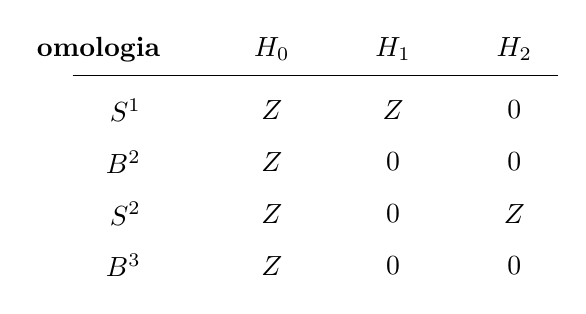
\begin{tikzpicture}[scale=1.1]
        \node at (0,2.3) {\textbf{omologia}};
        \node at (2.0,2.3) {$H_0$}; \node at (3.4,2.3) {$H_1$}; \node at (4.8,2.3) {$H_2$};
        \node[left] at (0.6,1.6) {$S^1$}; \node at (2.0,1.6) {$\mathbb{Z}$}; \node at (3.4,1.6) {$\mathbb{Z}$}; \node at (4.8,1.6) {$0$};
        \node[left] at (0.6,1.0) {$B^2$}; \node at (2.0,1.0) {$\mathbb{Z}$}; \node at (3.4,1.0) {$0$}; \node at (4.8,1.0) {$0$};
        \node[left] at (0.6,0.4) {$S^2$}; \node at (2.0,0.4) {$\mathbb{Z}$}; \node at (3.4,0.4) {$0$}; \node at (4.8,0.4) {$\mathbb{Z}$};
        \node[left] at (0.6,-0.2) {$B^3$}; \node at (2.0,-0.2) {$\mathbb{Z}$}; \node at (3.4,-0.2) {$0$}; \node at (4.8,-0.2) {$0$};
        \draw (-0.3,2.0) -- (5.3,2.0);
    \end{tikzpicture}
    \caption{Tabella riassuntiva dei gruppi di omologia di $S^1, B^2, S^2, B^3$.}
\end{figure}


% ======== NUOVO (pp. 183-186, 6/11) ========
\subsection{4) Il piano proiettivo $X = \mathbb{R}P^2$}

$\mathbb{R}P^2 = S^2/\{\pm\mathrm{Id}\}$ si rappresenta come un disco (o un quadrato) con i punti antipodali del bordo identificati. Triangolando il quadrato, si ottiene un complesso simpliciale $K$ con $\mathbb{R}P^2 = |K|$, che ha
\[
l_0 = 6 \ \text{($0$-simplessi)}, \qquad l_1 = 15 \ \text{($1$-simplessi)}, \qquad l_2 = 10 \ \text{($2$-simplessi)}.
\]

\begin{figure}[H]
    \centering
    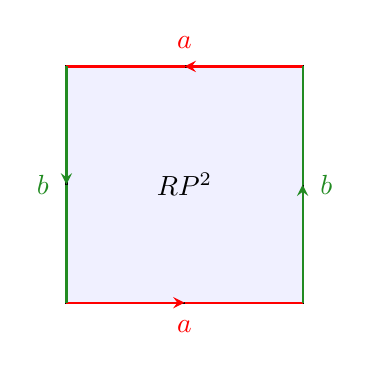
\begin{tikzpicture}[scale=1.0]
        \draw[thick, fill=blue!6] (0,0) rectangle (3,3);
        \draw[thick, red, ->, >=stealth] (0,0) -- (1.5,0); \draw[thick, red] (1.5,0) -- (3,0);
        \draw[thick, red, ->, >=stealth] (3,3) -- (1.5,3); \draw[thick, red] (1.5,3) -- (0,3);
        \draw[thick, ForestGreen, ->, >=stealth] (0,3) -- (0,1.5); \draw[thick, ForestGreen] (0,1.5) -- (0,0);
        \draw[thick, ForestGreen, ->, >=stealth] (3,0) -- (3,1.5); \draw[thick, ForestGreen] (3,1.5) -- (3,3);
        \node[red, below] at (1.5,-0.1) {$a$}; \node[red, above] at (1.5,3.1) {$a$};
        \node[ForestGreen, left] at (-0.1,1.5) {$b$}; \node[ForestGreen, right] at (3.1,1.5) {$b$};
        \node at (1.5,1.5) {$\mathbb{R}P^2$};
    \end{tikzpicture}
    \caption{Il piano proiettivo come quadrato con i lati identificati (parola $abab$ nel senso: i lati opposti sono identificati con orientazione opposta, cio\`e con una torsione).}
\end{figure}

\begin{itemize}
    \item $H_0(\mathbb{R}P^2, \mathbb{Z}) = \mathbb{Z}$ (connesso).
    \item $H_1(\mathbb{R}P^2, \mathbb{Z}) = \Pi_1(\mathbb{R}P^2)/\Pi_1(\mathbb{R}P^2)' = \mathbb{Z}_2$ (perch\'e $\Pi_1(\mathbb{R}P^2) \cong \mathbb{Z}_2$ \`e abeliano). Osserviamo che $H_1(\mathbb{R}P^2, \mathbb{Z}) = 0 \oplus \mathbb{Z}_2$: la parte libera \`e nulla (rango $0$) e tutta la torsione \`e $\mathbb{Z}_2$.
    \item $H_2(\mathbb{R}P^2, \mathbb{Z}) = 0$. (Vedremo che $H_2(\mathbb{R}P^2, \mathbb{R}) = 0$; poich\'e $H_2(K, \mathbb{Z}) = Z_2(K, \mathbb{Z})$ \`e un sottogruppo del gruppo libero $C_2(K, \mathbb{Z})$, \`e libero, dunque se ha rango $0$ \`e nullo.)
\end{itemize}

\begin{intuizione}
$H_1(\mathbb{R}P^2) = \mathbb{Z}_2$ \`e il primo esempio di \emph{torsione}: la ``retta proiettiva'' $\mathbb{R}P^1 \subset \mathbb{R}P^2$ non \`e un bordo, ma $2 \cdot \mathbb{R}P^1$ \`e il bordo dell'intera $\mathbb{R}P^2$ (cio\`e del disco), e dunque rappresenta un elemento di ordine $2$.
\end{intuizione}

\section{La caratteristica di Eulero--Poincar\'e}

\begin{definicion}[Caratteristica di Eulero--Poincar\'e]
Sia $K$ un complesso simpliciale di dimensione $m$ e sia $b_p = \dim H_p(K, \mathbb{R}) = \operatorname{rango}\big(\beta_p(K, \mathbb{Z})\big)$ ($p = 0, \dots, m$) il $p$-esimo numero di Betti. Si chiama \textbf{caratteristica di Eulero--Poincar\'e} di $K$ il numero
\[
\chi(K) = \sum_{p=0}^m (-1)^p\, b_p(K) .
\]
\end{definicion}

\begin{observacion}
$\chi$ \`e un \textbf{invariante topologico}: se $X$ \`e uno spazio triangolabile, $X = |K|$, allora $\chi(X) = \chi(K)$ (non dipende dalla triangolazione, perch\'e i numeri di Betti sono invarianti per omeomorfismo).
\end{observacion}

\begin{lema}
Sia $K$ un complesso simpliciale e $l_p$ il numero dei $p$-simplessi di $K$. Allora
\[
b_p(K) = \dim Z_p(K, \mathbb{R}) + \dim Z_{p+1}(K, \mathbb{R}) - l_{p+1} .
\]
\end{lema}
\begin{proof}
$b_p(K) = \dim H_p(K, \mathbb{R}) = \dim \dfrac{Z_p(K,\mathbb{R})}{B_p(K, \mathbb{R})} = \dim Z_p(K, \mathbb{R}) - \dim B_p(K, \mathbb{R}) = \dim Z_p(K, \mathbb{R}) - \dim \operatorname{Im} \partial_{p+1}$.
Ora $\partial_{p+1}: C_{p+1}(K, \mathbb{R}) \to C_p(K, \mathbb{R})$ \`e lineare e $\dim C_{p+1}(K, \mathbb{R}) = l_{p+1}$; per il teorema nullit\`a $+$ rango,
\[
l_{p+1} = \dim \operatorname{Ker} \partial_{p+1} + \dim \operatorname{Im} \partial_{p+1} = \dim Z_{p+1}(K, \mathbb{R}) + \dim \operatorname{Im} \partial_{p+1} .
\]
Quindi $\dim \operatorname{Im} \partial_{p+1} = l_{p+1} - \dim Z_{p+1}$ e sostituendo si ottiene la tesi\hfill$\square$
\end{proof}

\begin{teo}[di Eulero--Poincar\'e]
Sia $K$ un complesso simpliciale, $m = \dim K$ e $l_p$ il numero di $p$-simplessi di $K$. Allora
\[
\chi(K) = \sum_{p=0}^m (-1)^p\, l_p .
\]
\end{teo}
\begin{proof}
Per il lemma (con la convenzione $Z_{m+1} = 0$, $l_{m+1} = 0$):
\[
\chi(K) = \sum_{p=0}^m (-1)^p b_p = \sum_{p=0}^m (-1)^p \dim Z_p + \sum_{p=0}^m (-1)^p \dim Z_{p+1} - \sum_{p=0}^m (-1)^p l_{p+1} .
\]
Con il cambio di indice $q = p+1$ nei due ultimi termini:
\[
\chi(K) = \sum_{p=0}^m (-1)^p \dim Z_p + \sum_{q=1}^m (-1)^{q-1} \dim Z_q - \sum_{q=1}^m (-1)^{q-1} l_q .
\]
Nella prima somma separiamo il termine $p = 0$: $\sum_{p=0}^m (-1)^p \dim Z_p = \dim Z_0 + \sum_{p=1}^m (-1)^p \dim Z_p$. La seconda somma, $\sum_{q=1}^m (-1)^{q-1} \dim Z_q = -\sum_{q=1}^m (-1)^q \dim Z_q$, cancella esattamente la parte $\sum_{p=1}^m (-1)^p \dim Z_p$. Rimane $\dim Z_0 = l_0$ (perch\'e $\partial_0 = 0$), e il terzo termine vale $-\sum_{q=1}^m (-1)^{q-1} l_q = \sum_{q=1}^m (-1)^q l_q$. Dunque
\[
\chi(K) = l_0 + \sum_{q=1}^m (-1)^q l_q = \sum_{p=0}^m (-1)^p l_p . \qquad \square
\]
\end{proof}

\begin{intuizione}
Per un poliedro ``classico'' ($l_0$ vertici, $l_1$ spigoli, $l_2$ facce) si ritrova la formula di Eulero $V - E + F$. Il teorema dice che questo numero \emph{non dipende dalla triangolazione}, perch\'e coincide con $\sum (-1)^p b_p$, che \`e un invariante topologico.
\end{intuizione}

\begin{ejemplo}
\begin{enumerate}
    \item \textbf{$\chi(S^1)$.} Sappiamo che $H_0(S^1, \mathbb{R}) = \mathbb{R}$ ($b_0 = 1$) e $H_1(S^1, \mathbb{R}) = \mathbb{R}$ ($b_1 = 1$), quindi $\chi(S^1) = b_0 - b_1 = 1 - 1 = 0$. Verifica: $S^1 = |K|$, $K = [v_0, v_1, v_2]^1$, $l_0 = 3$, $l_1 = 3$, quindi per il teorema di Eulero--Poincar\'e $\chi(S^1) = \chi(K) = 3 - 3 = 0$.
    \item \textbf{$\chi(B^2)$.} $K = [v_0, v_1, v_2]$ con $l_0 = 3$, $l_1 = 3$, $l_2 = 1$: $\chi(B^2) = 3 - 3 + 1 = 1$. Verifica: $H_0(B^2, \mathbb{R}) = \mathbb{R}$ ($b_0 = 1$), $H_1(B^2, \mathbb{R}) = H_2(B^2, \mathbb{R}) = 0$ ($b_1 = b_2 = 0$), quindi $\chi(B^2) = 1 - 0 + 0 = 1$.
    \item \textbf{$\chi(\mathbb{R}P^2)$.} Con la triangolazione precedente, $\chi(\mathbb{R}P^2) = 6 - 15 + 10 = 1$.
\end{enumerate}
\end{ejemplo}

\begin{teo}
Sia $p: \widetilde{X} \to X$ un'applicazione di rivestimento ad un numero finito $h$ di fogli. Se $X$ \`e triangolabile, allora $\widetilde{X}$ \`e triangolabile e
\[
\chi(\widetilde{X}) = h \cdot \chi(X) .
\]
\end{teo}


% ======== NUOVO (pp. 187-192, 6/11) ========
\begin{ejemplo}[Altri calcoli di $\chi$]
\begin{enumerate}
    \item[3)] \textbf{$\chi(S^2)$.} $S^2 = |K|$ con $K = [v_0, v_1, v_2, v_3]^2$: $l_0 = 4$, $l_1 = 6$, $l_2 = 4$, quindi $\chi(S^2) = 4 - 6 + 4 = 2$. Infatti $\chi(S^2) = b_0 - b_1 + b_2 = 1 - 0 + 1 = 2$.
    \item[4)] \textbf{$\chi(\mathbb{R}P^2)$ e $H_2(\mathbb{R}P^2, \mathbb{R})$.} Con la triangolazione di $\mathbb{R}P^2$ ($l_0 = 6$, $l_1 = 15$, $l_2 = 10$) si ha $\chi(\mathbb{R}P^2) = 6 - 15 + 10 = 1$. Allora $1 = \chi(\mathbb{R}P^2) = b_0 - b_1 + b_2 = 1 - 0 + b_2$ (qui $b_1 = 0$ perch\'e $H_1(\mathbb{R}P^2, \mathbb{Z}) = \mathbb{Z}_2$ ha rango $0$), da cui $b_2 = 0$, cio\`e $H_2(\mathbb{R}P^2, \mathbb{R}) = 0$.
    \item[5)] \textbf{$\chi(T^2)$ e $H_2(T^2, \mathbb{R})$.} Il toro \`e triangolabile: $T^2 = |K|$ con (ad esempio) $l_0 = 16$, $l_1 = 48$, $l_2 = 32$ (si triangola il quadrato con i lati identificati). Quindi $\chi(T^2) = 16 - 48 + 32 = 0$. Allora $0 = \chi(T^2) = b_0 - b_1 + b_2$ con $b_0 = 1$ ($T^2$ \`e connesso) e $H_1(T^2, \mathbb{Z}) = \Pi_1(T^2) = \mathbb{Z}^2$ (abeliano), dunque $b_1 = 2$. Ne segue $0 = 1 - 2 + b_2$, cio\`e $b_2 = 1$ e $H_2(T^2, \mathbb{R}) = \mathbb{R}$.
\end{enumerate}
\end{ejemplo}

\begin{figure}[H]
    \centering
    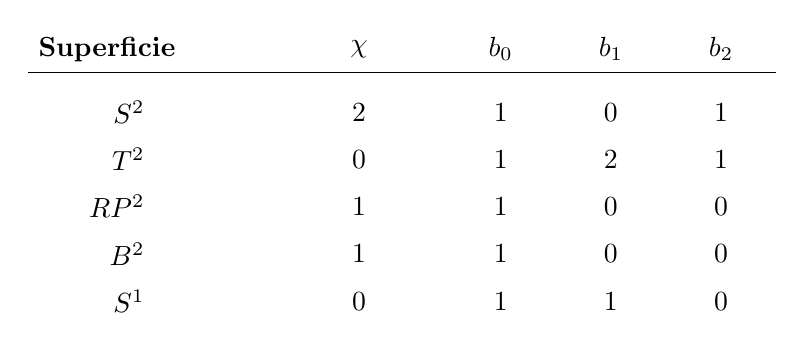
\begin{tikzpicture}[scale=1.0]
        \node at (0,3.3) {\textbf{Superficie}};
        \node at (3.2,3.3) {$\chi$}; \node at (5.0,3.3) {$b_0$}; \node at (6.4,3.3) {$b_1$}; \node at (7.8,3.3) {$b_2$};
        \draw (-1,3.0) -- (8.5,3.0);
        \node[left] at (0.6,2.5) {$S^2$}; \node at (3.2,2.5) {$2$}; \node at (5.0,2.5) {$1$}; \node at (6.4,2.5) {$0$}; \node at (7.8,2.5) {$1$};
        \node[left] at (0.6,1.9) {$T^2$}; \node at (3.2,1.9) {$0$}; \node at (5.0,1.9) {$1$}; \node at (6.4,1.9) {$2$}; \node at (7.8,1.9) {$1$};
        \node[left] at (0.6,1.3) {$\mathbb{R}P^2$}; \node at (3.2,1.3) {$1$}; \node at (5.0,1.3) {$1$}; \node at (6.4,1.3) {$0$}; \node at (7.8,1.3) {$0$};
        \node[left] at (0.6,0.7) {$B^2$}; \node at (3.2,0.7) {$1$}; \node at (5.0,0.7) {$1$}; \node at (6.4,0.7) {$0$}; \node at (7.8,0.7) {$0$};
        \node[left] at (0.6,0.1) {$S^1$}; \node at (3.2,0.1) {$0$}; \node at (5.0,0.1) {$1$}; \node at (6.4,0.1) {$1$}; \node at (7.8,0.1) {$0$};
    \end{tikzpicture}
    \caption{Tabella di caratteristiche di Eulero e numeri di Betti ($\chi = b_0 - b_1 + b_2$).}
\end{figure}

\begin{ejercicio*}
Calcolare $\chi(S^1 \vee S^1)$ e $\chi(S^1 \vee S^2)$.
\end{ejercicio*}
\textit{Soluzione.} Per $S^1 \vee S^1$ (due triangoli vuoti con un vertice in comune): $l_0 = 5$, $l_1 = 6$, $\chi = 5 - 6 = -1$ (conferma: $b_0 = 1$, $b_1 = 2$, $\chi = 1 - 2 = -1$). Per $S^1 \vee S^2$ si usa $b_0 = 1$, $b_1 = 1$, $b_2 = 1$: $\chi = 1 - 1 + 1 = 1$.

\begin{teo}
Per ogni $n \geqslant 1$:
\[
\chi(S^n) = \begin{cases} 0 & \text{se } n \text{ \`e dispari}, \\ 2 & \text{se } n \text{ \`e pari}. \end{cases}
\]
Inoltre $\chi(B^n) = 1$ per ogni $n$.
\end{teo}
\begin{proof}
$S^n$ \`e triangolabile: $S^n = |K|$ dove $K$ \`e l'$n$-scheletro di un $(n+1)$-simplesso (che ha $\binom{n+2}{p+1}$ simplessi di dimensione $p$). Per il teorema di Eulero--Poincar\'e,
\[
\begin{aligned}
\chi(S^n) = \chi(K) &= \sum_{p=0}^n (-1)^p \binom{n+2}{p+1} = - \sum_{q=1}^{n+1} (-1)^q \binom{n+2}{q} \\
&= - \Big( \underbrace{\sum_{q=0}^{n+2} (-1)^q \binom{n+2}{q}}_{=(1-1)^{n+2} = 0} - 1 - (-1)^{n+2} \Big) = 1 + (-1)^n ,
\end{aligned}
\]
che vale $0$ se $n$ \`e dispari e $2$ se $n$ \`e pari. Inoltre $B^n = |K'|$ con $K'$ un $n$-simplesso chiuso, che ha $\binom{n+1}{p+1}$ simplessi di dimensione $p$:
\[
\chi(B^n) = \sum_{p=0}^n (-1)^p \binom{n+1}{p+1} = \sum_{p=0}^{n-1} (-1)^p \binom{n+1}{p+1} + (-1)^n = \chi(S^{n-1}) + (-1)^n = 1 \quad \forall n .
\]
(se $n$ \`e dispari: $\chi(S^{n-1}) + (-1)^n = 2 - 1 = 1$; se $n$ \`e pari: $0 + 1 = 1$.)\hfill$\square$
\end{proof}

\begin{observacion}
Si pu\`o anche scrivere $B^n = \partial B^n \sqcup \mathring{B}^n = S^{n-1} \sqcup \{ (v_0, \dots, v_n) \}$ (il bordo pi\`u l'unico $n$-simplesso aperto, di segno $(-1)^n$): quindi $\chi(B^n) = \chi(S^{n-1}) + (-1)^n = 1$.
\end{observacion}

\begin{coro}
\[
\chi(\mathbb{R}P^n) = \begin{cases} 0 & \text{se } n \text{ \`e dispari}, \\ 1 & \text{se } n \text{ \`e pari}. \end{cases}
\]
\end{coro}
\begin{proof}
$S^n \to \mathbb{R}P^n$ \`e un rivestimento a $h = 2$ fogli, quindi $\chi(S^n) = 2\,\chi(\mathbb{R}P^n)$ per il teorema sulle caratteristiche dei rivestimenti, da cui $\chi(\mathbb{R}P^n) = \chi(S^n)/2 = 0$ ($n$ dispari) oppure $1$ ($n$ pari)\hfill$\square$
\end{proof}

\begin{observacion}[Idea della dimostrazione di $\chi(\widetilde{X}) = h\,\chi(X)$]
Se $K$ \`e una triangolazione di $X$, dopo un numero sufficiente di suddivisioni baricentriche ogni simplesso \`e contenuto in un aperto ben coperto (numero di Lebesgue). Poich\'e un simplesso \`e semplicemente connesso, si solleva in $h$ simplessi disgiunti di $\widetilde{X}$. Si ottiene una triangolazione di $\widetilde{X}$ con $\widetilde{l}_p = h\, l_p$ simplessi in ogni dimensione, e quindi $\chi(\widetilde{X}) = \sum (-1)^p h\, l_p = h\,\chi(X)$. (Questo spiega anche perch\'e $\chi(S^n) = 2\chi(\mathbb{R}P^n)$.)
\end{observacion}

\section{La formula di Eulero per i poliedri}

\begin{definicion}[Poliedro]
Un \textbf{poliedro} di $\mathbb{R}^3$ \`e un sistema finito di poligoni, giacenti su piani distinti, disposti in modo tale che in ogni spigolo si incontrino due facce, e che sia possibile passare da uno di tali poligoni a qualunque altro esclusivamente oltrepassando degli spigoli. Un poliedro $P$ si dice (metricamente) \textbf{regolare} se \`e formato da poligoni regolari congruenti tra loro; si dice \textbf{convesso} se lo \`e (come insieme di punti); si dice \textbf{semplice} se (come insieme di punti) \`e omeomorfo a $S^2$.
\end{definicion}

\begin{observacion}
Un poliedro convesso \`e semplice (omeomorfo a $S^2$ per proiezione radiale da un punto interno) e un poliedro semplice \`e in particolare un poliedro; i viceversa sono falsi (ad esempio un poliedro non convesso, o un toro poliedrico, che non \`e omeomorfo a $S^2$). I solidi platonici (poliedri regolari convessi) sono semplici. Inoltre ogni poligono \`e triangolabile, quindi ogni poliedro \`e triangolabile.
\end{observacion}

\begin{teo}[Formula di Eulero]
Sia $P$ un poliedro semplice e siano $V$, $S$, $F$ rispettivamente il numero di vertici, spigoli e facce di $P$. Allora
\[
V - S + F = 2 .
\]
\end{teo}
\begin{proof}
$P$ semplice $\Rightarrow$ $P \cong S^2$ $\Rightarrow$ $\chi(P) = \chi(S^2) = 2$. Senza perdere generalit\`a si pu\`o assumere $P$ convesso (per ogni poliedro semplice esiste un poliedro convesso con gli stessi $V$, $S$, $F$: la formula \`e puramente combinatoria). Indichiamo con $F_i$ ($i = 1, \dots, k$) il numero di facce di $P$ con $r_i$ lati; $F_1 + \dots + F_k = F$. Essendo $P$ convesso, ogni poligono di $P$ \`e convesso e, se ha $r_i$ lati, si pu\`o triangolare aggiungendo $(r_i - 3)$ diagonali uscenti da un suo vertice fissato.

\begin{figure}[H]
    \centering
    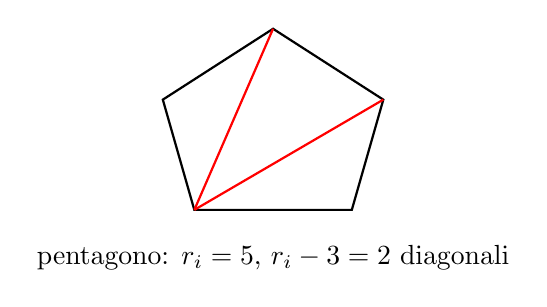
\begin{tikzpicture}[scale=1.0]
        \draw[thick] (0,0) -- (2,0) -- (2.4,1.4) -- (1,2.3) -- (-0.4,1.4) -- cycle;
        \draw[thick, red] (0,0) -- (2.4,1.4); \draw[thick, red] (0,0) -- (1,2.3);
        \node at (1,-0.6) {pentagono: $r_i = 5$, $r_i - 3 = 2$ diagonali};
    \end{tikzpicture}
    \caption{Triangolazione di una faccia convessa con $r_i - 3$ diagonali uscenti da un vertice.}
\end{figure}

Dunque $P = |K|$, dove $K$ \`e il complesso simpliciale ottenuto da $P$ aggiungendo le diagonali sui poligoni di $P$. Per il teorema di Eulero--Poincar\'e, $2 = \chi(P) = \chi(K) = l_0 - l_1 + l_2$ con $l_0 = V$, $l_1 = S + \sum_{i=1}^k (r_i - 3)F_i$, $l_2 = \sum_{i=1}^k (r_i - 2)F_i$. Perci\`o
\[
2 = V - S - \sum_i (r_i - 3)F_i + \sum_i (r_i - 2)F_i = V - S + \sum_{i=1}^k F_i = V - S + F. \qquad \square
\]
\end{proof}

\begin{teo}[Poliedri regolari]
Esistono esattamente $5$ classi distinte di poliedri regolari: tetraedro, cubo, ottaedro, dodecaedro e icosaedro.
\end{teo}
\begin{proof}[Dimostrazione (le condizioni necessarie)]
Sia $P$ regolare. Allora $P$ \`e semplice, quindi $V - S + F = 2$. Inoltre, essendo $P$ regolare, a ogni vertice converge lo stesso numero $n$ di spigoli, e ogni faccia ha lo stesso numero $r$ di lati. Contando le coppie (vertice, spigolo) e (faccia, spigolo): $nV = 2S$ e $rF = 2S$, cio\`e $V = 2S/n$ e $F = 2S/r$. Sostituendo nella formula di Eulero:
\[
\frac{2S}{n} - S + \frac{2S}{r} = 2 \implies \frac1n - \frac12 + \frac1r = \frac1S .
\]
Per il loro significato geometrico $n \geqslant 3$ e $r \geqslant 3$. Non pu\`o essere contemporaneamente $n \geqslant 4$ e $r \geqslant 4$: altrimenti $\frac1S = \frac1n - \frac12 + \frac1r \leqslant \frac14 - \frac12 + \frac14 = 0$, assurdo. Quindi $n = 3$ oppure $r = 3$.
\begin{itemize}
    \item $n = 3$: $\frac1S = \frac13 - \frac12 + \frac1r = \frac{6 - r}{6r} > 0$ implica $r < 6$, cio\`e $r \in \{3, 4, 5\}$.
    \item $r = 3$: analogamente $n \in \{3, 4, 5\}$.
\end{itemize}
Le coppie possibili $(n, r)$ sono dunque $(3,3), (3,4), (3,5), (4,3), (5,3)$, corrispondenti rispettivamente a tetraedro, cubo, dodecaedro, ottaedro e icosaedro (ciascuna esiste ed \`e unica a meno di similitudine)\hfill$\square$
\end{proof}

\begin{figure}[H]
    \centering
    \begin{tabular}{l|c|c|c|c|c}
    \textbf{Solido} & $n$ (spigoli per vertice) & $r$ (lati per faccia) & $V$ & $S$ & $F$ \\ \hline
    Tetraedro & 3 & 3 & 4 & 6 & 4 \\
    Cubo & 3 & 4 & 8 & 12 & 6 \\
    Ottaedro & 4 & 3 & 6 & 12 & 8 \\
    Dodecaedro & 3 & 5 & 20 & 30 & 12 \\
    Icosaedro & 5 & 3 & 12 & 30 & 20 \\
    \end{tabular}
    \caption{I cinque solidi platonici: in ogni caso $V - S + F = 2$.}
\end{figure}


